%%%%%%%%%%%%%%%%%%%%%%%%%%%%%%%%%%%%%%%%%%%%%%%%%%%%%%%%%%%
%% Congratulations, you've made an excellent choice
%% of writing your Tampere University thesis using
%% the LaTeX system. This document attempts to be
%% as complete a template as possible to let you focus
%% on the most important part: the writing itself.
%% Thus the details regarding the visual appearance
%% and even structure have already been worked out
%% for you!
%%
%% I sincerely hope you will find this template useful
%% in completing your thesis project. I've tried to
%% add comments (followed by the % sign) to clarify
%% the structure and purpose of some of the commands.
%% Most of the magic happens in the file tauthesis.cls,
%% which you are more than welcome to take a look at.
%% Just refrain from editing it in the most crucial
%% versions of the thesis!
%%
%% I wish you and your thesis project the best of luck!
%% If this template causes you trouble along the way
%% or if you've any suggestions for improving it,
%% please be in contact through GitHub
%% (<URL HERE>)
%%
%% Yours,
%%
%% Ville Koljonen
%%
%% PS. This template or its associated class file don't
%% come with a warranty. The content is provided as is,
%% without even the implied promise of fitness to the
%% mentioned purpose. You, as the author of the thesis,
%% are responsible for the entire work, including the
%% provided material. No one else is liable to you for
%% any damage inflicted on you or your thesis, were it
%% caused by using this template or not.
%%%%%%%%%%%%%%%%%%%%%%%%%%%%%%%%%%%%%%%%%%%%%%%%%%%%%%%%%%%

%%%%% NOTICE %%%%%
%% Please read through the entire template
%% (files under ./tex) to find all instructions.
%% It is possible that the attached pdf files
%% do not include the latest information.
%%%%%%%%%%%%%%%%%%

%%%%% INSTRUCTIONS FOR COMPILING THE DOCUMENT %%%%%
%% Overleaf: just click Recompile.
%% Terminal:
%%  1. pdflatex main.tex
%%  2. makeindex -s main.ist -t main.glg -o main.gls main.glo
%%  3. biber main
%%  4. pdflatex main.tex
%%  5. pdflatex main.tex
%% Similar sequence of commands is also required
%% in LaTeX specific editors.
%%%%%%%%%%%%%%%%%%%%%%%%%%%%%%%%%%%%%%%%%%%%%%%%%%%

%%% Set PDF version before doing anything else.

%%% set-pdf-version.tex
%
% This file is loaded by main.tex before any other operations, so that PDF
% version is set correctly for accessibility features.
%

\RequirePackage{ifluatex}

\def\mypdfminorversion{6}

\ifluatex

    \directlua {
        if pdf.getminorversion() \string~= \mypdfminorversion then
            if (status.pdf_gone and status.pdf_gone > 0)
            or (status.pdf_ptr and status.pdf_ptr > 0)
            then
                tex.error("PDF version cannot be changed anymore.")
            else
                pdf.setminorversion(\mypdfminorversion)
            end
        end
    }

\else

    \pdfminorversion=\mypdfminorversion

\fi


%%%%% METADATA %%%%%
%
% Always keep the following metadata up to date! This is important for your
% PDF file to comply to accessibility standards. (And yes, this information
% must remain here, before \documentclass[...]{...}.)

\def\myfititle{Kielimallien käyttäminen tapahtumasuunnittelussa}
\def\myentitle{A Descriptive title}
\def\myauthor{Ville Nupponen}
\def\myfisubtitle{Onko kielimalli mahdollista integroida yksinkertaisesti osaksi sovellusta ja saada tuottamaan haluttu lopputus?}
\def\myensubtitle{}
\def\myfithesistype{Diplomityö}
\def\myenthesistype{Master's thesis}
\def\myexaminers{Professori Hannu-Matti Järvinen \\ Kappalainen Timo Kälviäinen}
\def\myfifacultyname{Informaatioteknologian ja viestinnän tiedekunta}
\def\myenfacultyname{Faculty of Information Technology and Communication Sciences}
\def\myfiprogrammename{Tietotekniikka}
\def\myenprogrammename{Computing Sciences}
\def\myfikeywords{kielimalli, tekoäly, AI, Gemini, PaLM, Llama, Claude, xAI, rippileiri}
\def\myenkeywords{}
\def\mylanguagecode{fi-FI}
\def\mysubject{}
\def\myyear{2025}
\def\mymonth{02}
\def\myday{07}

% Define your citation options here. Valid values for style and sorting options
% can be found in the BibLaTeX manual: https://ctan.org/pkg/biblatex.

\def\mycitationstyle{numeric}
\def\mycitationsorting{nyt}

%%%%% PREAMBLE %%%%%

%%%%% Document class declaration.
%
% The possible optional arguments are
%
%   finnish - thesis in Finnish (default)
%   english - thesis in English
%   draft - for faster non-final works, also skips images
%           (recommended, remove in final version)
%   programs - if you wish to display code snippets
% Example: \documentclass[english, authoryear]{tauthesis}
%          thesis in English with author-year citations

\documentclass[finnish]{tauthesis}

%%% preamble.tex
%
% This file is for including LaTeX libraries or packages and defining your own
% commands.
%
% NOTE: The glossaries package loaded by tauthesis.cls throws a warning: No
% language module detected for 'finnish'. You can safely ignore this. All
% other warnings should be taken care of, before your thesis is submitted!

%%%%% Your packages.
%
% Before adding packages, see if they can be found in tauthesis.cls already.
% If you're not sure that you need a certain package, don't include it in the
% document! This can dramatically reduce compilation time.

% Graphs
% \usepackage{pgfplots}
% \pgfplotsset{compat=1.15}

% Subfigures and wrapping text
% \usepackage{subcaption}

%% Theorem environments and their numbering.
%
% Define both English and Finnish theorem types. These all follow the same
% counter. See the documentation of amsthm to see how these can be changed to
% suit your needs, if necessary.
%

\usepackage{amsthm}

\theoremstyle{definition}

%\newtheorem{definition}{Definition}[chapter]
%\newtheorem{theorem}[definition]{Theorem}

%\newtheorem{maaritelma}[definition]{Määritelmä}
%\newtheorem{lause}[definition]{Lause}

% Mathematics packages
\usepackage{mathtools, amssymb}
%\usepackage{bm}

% Chemistry packages
% \usepackage{chemfig}
% \usepackage[version=4]{mhchem}

% Text hyperlinking
% \usepackage{hyperref}
% \hypersetup{hidelinks}

% (SI) unit handling
% \usepackage{siunitx}

%\sisetup{
%    detect-all,
%    math-sf=\mathrm,
%    exponent-product=\cdot,
%    output-decimal-marker={,} % for theses in FINNISH!
%}

%%%%% Your commands.

% Print verbatim LaTeX commands
\newcommand{\verbcommand}[1]{\texttt{\textbackslash #1}}

% Command for formatting code.

\newcommand\code[1]{\texttt{#1}}

% Basic theorems in Finnish and in English.
% Remove [chapter] if you wish a simply
% running enumeration.
% \newtheorem{lause}{Lause}[chapter]
% \newtheorem{theorem}[lause]{Theorem}

% \newtheorem{apulause}[lause]{Apulause}
% \newtheorem{lemma}[lause]{Lemma}

% Use these versions for individually
% enumerated lemmas
% \newtheorem{apulause}{Apulause}[chapter]
% \newtheorem{lemma}{Lemma}[chapter]

% Definition style
% \theoremstyle{definition}
% \newtheorem{maaritelma}{Määritelmä}[chapter]
% \newtheorem{definition}[maaritelma]{Definition}
% examples in this style

%%%%% Glossary information.

% Use the following lines ONLY if you need more
% than one glossary. The first argument specifies
% a type label for the glossary and the second
% the displayed name.
% \newglossary*{symbs}{Symbols}
% \newglossary{label}{Displayed name}
% ...

\makeglossaries

% Use this line if using the default glossary.
% Otherwise comment out.

\loadglsentries[main]{tex/sanasto.tex}

% Use this line if using more than one glossary.
% Otherwise comment out.
% \loadglsentries[symbs]{tex/sanasto2.tex}

%%%%% Citation information.

% Commonly used bibliography modifications.
% Feel free to play around with them.

%\ExecuteBibliographyOptions{%
%sorting=none,
%maxbibnames=99,
%maxcitenames=2,
%giveninits=true,
%uniquename=init,
%sortcites,
%sortlocale=fin}

%\DefineBibliographyStrings{finnish}{%
%    in = {},
%    pages = {s.},
%    page = {s.}
%}
%\DefineBibliographyStrings{english}{%
%    in = {},
%    pages = {pp.},
%    page = {p.}
%}
%
%\DeclareNameAlias{sortname}{last-first}
%\DeclareNameAlias{author}{last-first}

%\DeclareFieldFormat[%
%    article,inbook,incollection,inproceedings,
%    patent,thesis,unpublished]{citetitle}{#1\isdot}
%\DeclareFieldFormat[%
%    article,inbook,incollection,inproceedings,
%    patent,thesis,unpublished]{title}{#1\isdot}
%\DeclareFieldFormat{pagetotal}{#1 \bibstring{page}}

%\AtBeginBibliography{\renewcommand*{\makelabel}[1]{#1\hss}}

%\DefineBibliographyExtras{english}{\let\finalandcomma=\empty}

\addbibresource{tex/references.bib}
 % You can add packages and define new commands in this file.

\begin{document}

%%%%% FRONT MATTER %%%%%

\frontmatter

%%%%% Thesis information and title page.

% Enable the use of @ character in command names.

\makeatletter

% The titles of the work. If there is no subtitle, leave the \myfisubtitle or
% \myensubtitle command arguments empty. Pass the title in the primary
% language as the first argument and its translation to the secondary language
% as the second.

\if@langenglish

    \title{\myentitle}{\myfititle}

\else

    \title{\myfititle}{\myentitle}

\fi

\if@langenglish

    \subtitle{\myensubtitle}{\myfisubtitle}

\else

    \subtitle{\myfisubtitle}{\myensubtitle}

\fi

% The author name.

\author{\myauthor}

% The examiner information. If your work has multiple examiners, replace with
%
%   \examiner[<label>]{<name> \\ <name>}
%
% where <label> is an appropriate (plural) label, e.g. Examiners or
% Tarkastajat, and <name>s are replaced by the examiner names, each on their
% separate line.

\examiner{\myexaminers}

% The finishing date of the thesis (YYYY-MM-DD).

\finishdate{\myyear}{\mymonth}{\myday}

% The type of the thesis (e.g. Kandidaatintyö or Master of Science Thesis) in
% the primary and the secondary languages of the thesis.

\if@langenglish

    \thesistype{\myenthesistype}{\myfithesistype}

\else

    \thesistype{\myfithesistype}{\myenthesistype}

\fi

% The faculty and degree programme names in the primary and the secondary
% languages of the thesis, respectively.

\if@langenglish

    \facultyname{\myenfacultyname}{\myfifacultyname}

\else

    \facultyname{\myfifacultyname}{\myenfacultyname}

\fi

\if@langenglish

    \programmename{\myenprogrammename}{\myfiprogrammename}

\else

    \programmename{\myfiprogrammename}{\myenprogrammename}

\fi

% The keywords of the thesis in the primary and the secondary languages of the
% thesis.

\if@langenglish

    \keywords{\myenkeywords}{\myfikeywords}

\else

    \keywords{\myfikeywords}{\myenkeywords}
\fi

% Make @ a regular letter again.

\makeatother

% Actually generate the title page based on the above commands.

\maketitle


%%%%% Abstracts and preface.
%
% Write the abstract(s) and the preface into a separate file for the sake of
% clarity. Pass the appropriate file name as the first argument to these
% commands. Put the \abstract in the primary language first and the
% \otherabstract in the secondary language second. Those who do not speak
% Finnish only need the first abstract. The second argument of the \preface
% command takes the place where the thesis was signed in.

\abstract{tex/tiivistelma.tex}

% \otherabstract{tex/abstract.tex}

\aidisclaimerinclusioncmd

% \preface{tex/alkusanat.tex}{Tampereella}

%%%%% Table of contents.

\tableofcontents

%%%%% Lists of figures, tables, listings and terms.
%
% Print the lists of figures and/or tables. Uncomment either of these commands
% as required. Both are optional, but if there are many important
% figures/tables, listing them may be a good idea.

% \listoffigures
% \listoftables
% \lstlistoflistings

% Misc stuff related to how the glossary is displayed. You can especially
% tweak the lengths to suit you!

\glsaddall
\setglossarystyle{taulong}
\setlength{\glsnamewidth}{0.25\textwidth}
\setlength{\glsdescwidth}{0.75\textwidth}
\renewcommand*{\glsgroupskip}{}

% Print the default glossary of abbreviations, if necessary. Otherwise comment
% out. The appropriate Finnish variant is 'Lyhenteet'

\printglossary[title={Lyhenteet ja merkinnät}]

% Print more than one glossary with these lines. Otherwise comment out.

% \printglossary[type=symbs]
% \printglossary[type=label]
% ...

%%%%% MAIN MATTER %%%%%

\mainmatter

% Write each of the chapters of the thesis into a separate file for the sake
% of clarity. They can be \input as shown below. Give both the chapters and
% their files as descriptive names as possible.

\chapter{Johdanto}
\label{ch:johdanto}

Kielimallien käyttäminen on yleistynyt parin viime vuoden aikana huomattavasti
ja yhä useampi yritys ja organisaatio on ottanut kielimallit osaksi ellei jopa
kokonaan tulevaisuuden suunnitelmiksi. Isoilla teknologiajäteillä sekä suurelle
yleisölle ennen kielimallien suosion myötä saamaa julkisuutta hiukan
tuntemattomillakin teknologiafirmoilla on ollut jatkuva kilpailu siitä, kenen
kielimalli on kykenevin. Kielimalleja on vertailtu niin koulutettavan datan
määrällä kuin laitettu tekemään ihmisille suunnattuja tenttäjä tai muita kykyjä
mittaavia kokeita. Organisaatiorakenteitakin on pistetty uusiksi, jotta
kielimallien kehitys pystytään tekemään mahdollisimman tehokkaasti.

Tämän seurauksena tuleekin helposti kysymys: miten minä voisin käyttää
kielimalleja auttamaan tekemään niin sanotut raskaat työt? Voisiko kielimalli
luoda jotain luovaa nopeasti, jossa en ole itse onnistunut? Näiden kysymysten
pohtimiseen ja testaamiseen avautui sopiva tilaisuus kun eteen tuli tilanne,
jossa täytyi luoda nopeasti luovaa sisältöä ja muutaman henkilön parin tunnin
yrittämisen jälkeen ei sisältö ollut missään määrin kelvollista. Tässä työssä
onkin keskitytty luomaan työkalu, joka pyrkii estämään jatkossa kyseisen
tilanteen tapahtumisen. Työkalu tehdään osaksi diplomityön ohella tehtävää
sovellusta, joka pyrkii helpottamaan ja auttamaan seurakunnan rippileirin sekä
mahdollisesti muidenkin leirien vetäjien ja vapaaehtoisten koordinointia mm.
aikataulujen, vastuulistojen ja valmiiden materiaalien avulla.

Ensimmäisessä luvussa käydään lyhyesti läpi mitä kielimallit ovat, mitä niillä
voidaan nykyisin tehdä, miten niitä vertaillaan sekä lyhyesti katsotaan lyhyesti
kielimallien ja ylipäätään tekoälyn historiaa. Toisessa luvussa tuodaan esille
yleisiä tietoja muutamasta yleisestä kielimallilla, sekä lyhyt katsaus niiden
käytöstä ja hinnoittelusta, jotka vaikuttavat siihen, mitä kielimallia voidaan
lopullisessa toteutuksessa käyttää. Kolmannessa luvussa käydään läpi sovellusta,
siihen valittujen kielimallien integroinnin totutettamista sekä kevyt arviointi
kielimallien toimivuudesta.


\chapter{Kielimallit}
\label{ch:kielimallit}

Nykyisin tekoälystä kuulee jatkuvasti puhuttavan jossain muodossa. Tekoälyn
merkityksestä tulevaisuudella kuulee jatkuvasti erilaisia arvioita ja
intensiivinen ja nopea kehitys alalla avaa jatkuvasti yhä uusia
mahdollisuuksia. Se, että mikä on tekoäly, ei kuitenkaan ole täsmällisesti
määritelty ja yksi mahdollinen määritys voisi olla Työ- ja elinkeinoministeriön
julkaisussa käytettävä määritelmä "Tekoäly tarkoittaa laitteita, ohjelmistoja
ja järjestelmiä, jotka kykenevät oppimaan ja tekemään päätöksiä lähes samalla
tavalla kuin ihmiset. Tekoälyn avulla koneet, laitteet, ohjelmat, järjestelmät
ja palvelut voivat toimia tehtävän ja tilanteen mukaisesti järkevällä tavalla"
\parencite{valtioneuvostoSuomenTekoalyaika}.

Yhtenä keinoa toteuttaa tekoälyä voidaan käyttää kielimalleja. Kielimallit on
yleensä koulutettu ymmärtämään ja tuottamaan luonnollista kieltä. Tänä päivänä
paljon esillä olevat kielimallit ovat niin sanottuja suuria kielimalleja,
joiden koulutus on pohjautunut merkittävän suureen aineistoon. Ainoiston avulla
kielimallia voidaan opettaa ennustamaan, mitä sanoja tai lauseita aineistoin
mukaan annettaisiin vastauksena.

\section{Suuret kielimallit}

Suuret kielimallit tulivat tunnetuiksi suurelle osalle OpenAI:n marraskuussa
2022 julkaiseman ChatGPT-palvelun myötä tunnetuiksi
\parencite{alma9911564814005973}. Monille voikin tämän myötä jäädä kuva, että
kielimalleilta voi kysyä jotain ja ne tuottavat tekstiä vastauksena. Tätä monet
niistä tekevätkin, mutta tää päivänä käyttötarkoituksia on keksitty useita.
Perinteisen tekstin tuottamisen lisäksi kielimalleja käytetään mm. kuvan,
äänen ja videon tuottamiseen. Kielimalleja on yhdistelty ja ne voivatkin
ymmärtää useita eri syötteitä ja tuottaa tuloksia sen mukaan.

TODO: Mitä niillä ei voi tehdä? (strawberry esimerkki?)

\subsection{Tekstistä kuvaksi}

TODO: Imagen 3?
TODO: DALL-E 3?
TODO: Midjourney?
TODO: Stable diffusion?

\subsection{Tekstistä ääneksi}

TODO: https://suno.com/ ?
TODO: https://www.udio.com/ ?

\subsection{Tekstistä videoksi}

Helmikuussa 2024 OpenAi julkaisi Twitteriin useita tviittejä, jossa esiteltiin
lyhyitä videoita, jotka oli tuotettu antamalle Soralle, uudelle tekstistä
kuvaksi -mallille, lyhyehkö syöte siitä, mitä videossa halutaan tapahtuvan
\parencite{twitter1758192957386342435}. Ideana ei tuossa vaiheessa enää ollut
uutta, että toteutettaisiin videota tekstisyötteestä, mutta Soran tulokset
näyttivät, että se on todellakin mahdollista käytännössä eikä vain ideatasolla.

Soran kehityksen tautalla on ollut inspiraation ottaminen suurien kielimallien
toiminnasta. Suuret kielimallit on koulutettu internetin-laajuisella määrällä
tietoa ja LLM-paradigman menestys pohjautuukin tokeneihin. Vastaavasti Soralle
on kehitetty visuaalisia patcheja, joita on jo aiemmin nähty toimivan
visuaalisten toteutusten kanssa hyvin. Kuten suuret kielimallitkin, on Sora
tansformer-malli. Kuitenkin erona se, että Sora on nimenomaan diffuusio
transformer -malli. \parencite{openAISoraReport}

Soran kouluttamisessa on käytetty saatavilla olevaa dataa alkuperäisessä koossa
ilman leikkaamista vakiokokoisiksi. Tämä on yksi selvistä eroista verrattuna
muihin vastaaviin malleihin. Sen myötä on saatu useita etuja, kuten videoiten
tuottaminen eri kokoisina ja sisällön sijoittaminen paremmin näkyviin.
\parencite{openAISoraReport}

Kyseessä on tekstistä videoksi -malli, joten mallin on pelkän videon
tuottamisen lisäksi ymmärrettävä myös tekstiä. Tähän onkin Soran tapauksessa
käytetty OpenAI:n kehittämää tekniikkaa, jota DALL-E 3 käyttää. Myös GPT:n
avulla tekstisyötettä saadaan kuvailevammaksi ja mahdollistamaan sen myötä
parempien videoiden luontia. \parencite{openAISoraReport}

\section{Miten kielimalleja vertaillaan?}

Kielimallien määrän kasvaessa jatkuvasti on luonnollista, että kielimallit
kilpailevat siitä, mikä on paras kielimalli. Monien kielimallien julkaisuden
yhteydessä julkaistussa raportissa suurin osa sisällöstä onkin nimeen vertailua
ja statistiikkaa siitä miten kielimalli suoriutuu verrattuna muihin.
Raporteissa näkyvän vertailun voi jakaa kolmeen kategoriaan: kielimallien
vertailua aiempiin versioihin, kielimallien vertailua toisiin kielimalleihin
suorituskyvyn tai muun vastaavan mahdollisimman yksiselitteisen numerollisen
arvon avulla ja kielimallien vertailua erinäisten testien avulla, joilla
pyritään arvioimaan kielimallin kysyä mahdollisimman neutraalisti.

Kielimallien vertailuissa aiempiin malleihin Geminin kohdalla on toteutettu
useita eri suorituskykytestejä ja laskettu kuinka monessa testissä uudempi
versio on onnistunut paremmin ja sen myötä laskettu ns. voittosuhde. Näissä
suorituskykytestien määrä on vaihdellut ääniihin liittvien suorituskykytestien
viidestä aina tekstien 24 testiin ja keskeisten ominaisuuksien 50 testiin.
Määrät vaihtelevat myös riippuen minkä mallien välillä vertailua on tehty.
Helmikuun ja toukokuun mallien välisiä eroja on myös tarkemmin eroteltu
koostamalla kymmenkunta eri suorituskykytestiä ja testien antamia pisteitä
verrattu toisiinsa. \parencite{googleDeepmindGeminiv1_5report}

Geminin kohdalla on myös laskettu tehokkuutta mittaamalla sitä, minkä verran
kuluu keskimäärin aikaa yksittäiseen merkin tuottamiseen vastauksessa. Testissä
on annettu syötteitä englanniksi, japaniksi, kiinaksi ja ranskaksi. Mittaukset
on tehty käyttämällä Vertex AI:n ja OpenAI:n tarjoamia rajapintoja vertailteville
malleille. \parencite{googleDeepmindGeminiv1_5report} Tällä testillä on saatu
näkyviin niin sanottua raakaa dataa suorituskyvystä, mutta ottamatta kantaa
tuloksen varsiseen laatuun ja siten mallin suoriutumiseen. Vastaavia testejä
näkyykin huomattavasti vähemmän sillä ne eivät välttämättä yksinään kerra
malleista mitään.

Yksi Gemini 1.5:n merkittävimmistä asioista vaikuttaisi olevan Googlen
esityksen \parencite{googleKeynote2024} perusteella mahdollisuus merkittävästi
suurempaan kontekstiin. Tätä korostuu myös mallissa tehdyssä raportissa
\parencite{googleDeepmindGeminiv1_5report}, jossa vertailu keskittyy paljon
toimivuuteen suuremmilla konteksteilla. Monessa tapauskessa muilla malleilla ei
ole edes mahdollisuutta kyseisen kokoiseen kontekstiin, joten vertailut
keskittyvätkin pitkälti näyttämään miten mallien suoriutuminen kestää
kontekstin kasvamisen myötä.

Kun Gemini 1:n raportissa \parencite{googleDeepmindGeminiv1report} vertailtiin
muihin malleihin, on vertailu Gemini 1.5:n
\parencite{googleDeepmindGeminiv1report} tapauksessa Geminin eri versioiden
välillä. Geminin ollessa kykenevä useisiin eri asioihin, on myös
suorituskykytestejä usealla eri osa-alueella, kuten tekstin kohdalla
kyvykkyys matematiikassa, tieteessä ja päättelyssä, monikielisyydessä,
sekä koodauksessa. Visuaalisuuteen liittyen puolestaan multimodaaliessa
päättelyssä, kaavioiden ja dokumenttien käsittelyssä, kuvien luonnollisuuteen
sek videoiden ymmärtämiseen. Äänten kanssa puolestaan puheen tunnistamiseen ja
kääntämiseen.

Clauden uusimpien mallien, Claude 3.5 Sonnet ja Claude 3.5 Haiku kanssa on
esille tuotu erityisesti tiettyjen suorituskykytestien tuloksia. Näissä
testeissä on vertailtu tuloksia Clauden versioiden sekä GPT:n ja Geminin
vastaavien mallien välillä. \parencite{anthropicClaudeSonnetAndHaiku35}
\parencite{anthropicClaudeSonnet} \parencite{anthropicClaudeHaiku} Tuloksien
ymmärtäminen näistä voi olla selkeämpää verrattuna mm. Geminin raportteihin
\parencite{googleDeepmindGeminiv1report}
\parencite{googleDeepmindGeminiv1_5report}, mutta on vertailu on jätetty vain
yksittäisten suorituskykytestien tulosten varaan.

Suorituskykytestejä on eri kielimallien raportonneissa
\parencite{anthropicClaudeSonnetAndHaiku35} \parencite{openAI2023GPT4}
\parencite{openAIGPT4o} \parencite{googleDeepmindGeminiv1_5report} käytetty
lukuisia, mutta eniten esille tulevat MMMU, GPQA, MATH, HumanEval, MGSM ja
DROP, jotka ovat esitelty jokaisen tutkitun kielimallien suorituskyvyn
raportoinnissa. Näiden lisäksi on useita monet suorityskykytestit esiintyvät
useille eri malleilla. MMMU on suorituskykytesti, joka on suunniteltu
multimodaalisten mallien arviointiin massiivisiin, monialaisiin tehtäviin,
jotka vaativat korkeakoulutasoista tuntemusta ja päättelykykyä
\parencite{benchmarkMMMU}. GPQA on puolestaan kooste 448:sta haastavasta
monivalinta kysymyksestä biologian, fysiikan ja kemian alalla, johon tohtorin
tutkintoa tekevät saavat kaksi kolmasosaa oikein \parencite{benchmarkGPQA}.
Matemaattista ongelmanratkaisua mittaamaan on tehty MATH suorituskykyteksti,
jossa on 12 500 hasstavaa kilpamatematiikan ongelmaa, jotka sisältävät
kattavan vaihettaisin ratkaisun, jotta kielimallien kykyä johdatteluun ja
selittävään vastaukseen voidaan myös parantaa \parencite{benchmarkMATH}.
HumanEval \parencite{benchmarkHumanEval} on arviointoisarja, joka sisältää
164 käsinkirjoitettuja ohjelmointi ongelmaa. MSGM suorituskykytesti
pohjautuu 250 peruskoulutason matematiikan ongelmaan \parencite{benchmarkMSGM}.
DROP puolestaan on 96 000 kysymystä sisältävä testi englanninkielen
luetunymmärtämiselle, jotka pyrkii tuomaan haastetta sijoittelemalla
tarvittava tieto useisiin kohteisiin, joista on kyettävä yhdistelemään
lopullinen vastaus.

TODO: Missä kielimallit pärjäävät?
TODO: Missä kielimallit eivät pärjää?
TODO: Mitä eri luvut tarkoittavat? (mitä tarkoittaa jos koulutettu X määrällä dataa yms.)

\section{Historia \& tulevaisuus}

Tekoälyn historia alkaa 1950-luvun tienoilta, jolloin tänä päivänä tuntemamme
tietotekniikka oli vasta ihan alullaan. Ensimmäiset tekoälynratkaisut
suorittivat hyvin rajoitettuja tehtäviä, kuten ratkaisivat yksinkertaisia
matemaattisia laskutoimituksia. Vuonna 1956 järjestetyssä Dartmouth-
konferenssissa luotuun ehdotus, joka määäritteli perustavoitteet tekoälylle.
\parencite{alma9911564814005973}

1980-luvulla neuroverkot ja syväoppiminen avasivat uudenlaista potentiaalia
tekoälyille kun niiden nähtiin mahdollistavan muukin ratkaisu kuin vain
ohjelmistokehittäjän ennalta määrittämät tehtävät. Neuroverkoilla pyritään
matkikmaan ihmisten aivoja kun puolestaan syväoppimisella tuotiin useita
kerroksia, joissa jokainen kerros oppi datasta yhä monimutkaisempia piirteitä.
\parencite{alma9911564814005973}

Lähempänä nykypäivää käytettävissä olevan datan määrä on mahdollistanut sen
ettei tekoäly vain tekisi ihmisen määrittelemiä tehtäviä vaan kykenisi johonkin
oikeasti luovaan, kuten taiteeseen ja kirjoittamiseen.
\parencite{alma9911564814005973}

TODO: tulevaisuuden arvioita?


\chapter{Kielimallien vertailu}
\label{ch:vertailu}

Eri kielimalleja löytyy erittäin paljon ja variaatioita jo pelkästään yhdestä
kielimallista voi löytyä useita variaatioita. 2025 tammikuussa hakemalla
HuggingFacesta malleja rajoituksella "Text Generation", saadaan tuloksia lähes
170 000. Tässä työssä on tuotu esille joitain jossain määrin tunnetuimmista
kielimalleista isoimmilta tekijöiltä. Kielimallien tunnettavuutta korostaa muun
muassa se, että kielimallit esiintyvät toisten isojen kielimallien sivuilla ja
raporteissa vertailussa.

Varsinaisen toteutuksen kannalta rajoituksena on ensisijaisesti hinta. Koska
mallien toimintaa on tarkoitus vain testata, eikä ottaa pysyvään käyttöön, on
lähtökohtaisesti käytön mukainen hinnoittelu parempi. Tärkeänä kriteerinä on
myös se, että kielimallia on mahdollista saada käyttöön kohtuullisilla määrällä
työtä. Näiden kriteerien myötä valituista kielimalleista on esitelty
kielimallien perustiedot, toteutustapa sovellukseen ja hinnoittelu.

\section{Google Gemini}

Gemini on Googlen julkaisema kielimalliperhe, jonka on seuraaja PaLM 2:lle
\parencite{googleKeynote2023}. Googlella on myös Gemini-niminen ChatBot, joka
tunnettiin aiemmin nimellä Bard, ennen kuin Google nimesi sen uudelleen
Geminiksi \parencite{geminiUpdates}. Geministä on useita eri malleja, jotka on
tarkoitettu eri käyttötilanteisiin. Näitä malleja ovat Ultra, Pro, Flash ja
Nano. \parencite{googleDeepmindGemini} Näistä Ultra on tarkoitettu
monimutkaisimpiin tehtäviin, Pro optimoitu kustannusten ja viiveen kannalta ja
Nano puolestaan laitteissa pyöritettäväksi
\parencite{googleDeepmindGeminiv1report}. Flash puolestaan on entistä
kustannustehokkaampi ja nopeampi kuin Pro \parencite{googleKeynote2024}.
Malleista on useita eri versioita, jotka on välillä nimetty samoin kuin
edelliset versiot \parencite{googleDeepmindGeminiv1_5report}. Kehitys on ollut
erittäin nopeaa ja versiot vanhenevat nopeasti uusien tullessa käytettäviksi.

\subsection{Käyttö}

Gemini ei ole saatavilla Googlen AI Studion kautta ilman maksullista tilausta
Suomessa \parencite{googleAiAvailableRegions}. Geminiä on kuitenkin mahdollista
käyttää Vertex AI -alustan kautta.

Vertex AI -alustan käyttöön on tarjolla kirjastoja useille eri
ohjelmointikielille \parencite{vertexAiGenerativeAiQuickstart}. Luvussa
\ref{ch:sovellus} esitellyn sovelluksen taustajärjestelmä on toteutettu Javalla
ja pakettimanagerina on maven, joten Vertex AI:n Javalle tekemän kirjasto
saadaan käyttöön lisäämällä pom.xml-tiedostoon esimerkin
\ref{lst:vertexai-pom.xml} mukaisesti.

\begin{lstlisting}[
    basicstyle=\small,
    caption={google-cloud-vertexai riippuvuus pom.xml tiedostoon},
    label={lst:vertexai-pom.xml},
    language=xml,
]
<dependency>
    <groupId>com.google.cloud</groupId>
    <artifactId>google-cloud-vertexai</artifactId>
    <version>1.2.0</version>
</dependency>
\end{lstlisting}

Kevään 2024 aikana riippuvuuteen on tullut useita versioita, joista osa on
tuonut rikkovia muutoksia \parencite{mavenGoogleVertexAIAPI}. Kirjastoon
liittyvät koodit tässä työssä on tehty versiolle 1.2.0.

VertexAI:n kirjaston käyttäminen pohjautuu VertexAI-luokasta luotavaan
ilmiintymään, jota eri mallit käyttävät. Kyseinen ilmiintymä saadaan luotua
luomalla kohdan \ref{lst:AIConfig.java} mukaisesti VertexAI-bean, jonka myötä
ilmiintymää saadaan käytettyä Spring Frameworkin avulla helposti usealla eri
paikalla ilman, että konfiguraatio tarvitsee sotkea varsinaiseen toteutukseen
\parencite{baeldungSpringBean}.

\begin{lstlisting}[
    basicstyle=\small,
    caption={VertexAI konfiguraatio},
    label={lst:AIConfig.java},
    language=java,
]
// Merkitän luokka konfiguraatioksi, jotta Spring Framework saa
// käytetyä luokassa määriteltyjä asioita
@Configuration
public class AIConfig {

    // Luetaan ympäristömuuttujista VertexAI:n tarvitsema projekti
    // tunniste
    @Value("${VERTEX_AI_PROJECT_ID}")
    private String VERTEX_AI_PROJECT_ID;

    // Luetaan ympäristömuuttujista VertexAI:n tarvitsema rajapinnan
    // sijainti tieto
    @Value("${VERTEX_AI_LOCATION}")
    private String VERTEX_AI_LOCATION;

    // Luodaan VertexAI-bean ympäristömuuttujista luetuilla tiedoilla
    @Bean
    public VertexAI vertexAI() {
        return new VertexAI(VERTEX_AI_PROJECT_ID, VERTEX_AI_LOCATION);
    }
}
\end{lstlisting}

Konfiguraation jälkeen voidaan toteuttaa varsinainen Service, jossa kielimallia
käytetään. Esimerkki tällaisesta Servicestä on esitelty kohdassa
\ref{lst:GeminiServiceExample.java}.

\begin{lstlisting}[
    basicstyle=\small,
    caption={Esimerkki toteutus siitä, miten Geminiä voisi käyttää},
    label={lst:GeminiServiceExample.java},
    language=java,
]
// Merkitään luokka Serviceksi Spring Frameworkille
@Service
@RequiredArgsConstructor
public class GeminiService {

    private final VertexAI vertexAI;

    // Luodaan kielimallille konfiguraatio
    private GenerationConfig createGenerationConfig() {
        return GenerationConfig.newBuilder()
            .setMaxOutputTokens(2000)
            .build();
    }

    public void example() {
        // Luodaan ilmiintymä mallista
        GenerativeModel model =
            new GenerativeModel("gemini-1.0-pro", vertexAI);

        // Luodaan mallista Chat-istunto, jotta mallinan kanssa
        // voidaan jatkaa keskustelua
        ChatSession chatSession = model.startChat();

        // Annetaan istunnolle konfiguraatiot
        chatSession.withGenerationConfig(createGenerationConfig());

        // Lähetetään kielimallin kanssa luotuun chat-istuntoon
        // viesti "Kerro vitsi"
        GenerateContentResponse response =
            chatSession.sendMessage("Kerro vitsi");

        // Tulostetaan kielimallin vastaus
        System.out.println(response
            .getCandidates(0).getContent()
            .getParts(0).getText());
    }
}
\end{lstlisting}

\subsection{Hinnoittelu}

Gemini 1.0 Pron hinta syötteenä annetuille kuville on \$0.0025 / kuva, videolle
\$0.002 / sekunti, tekstille \$0.000125 / 1000 merkkiä ja ulostulolle
\$0.000375 / 1000 merkkiä. Gemini 1.5 Pron hinnat ovat noin puolet syötteelle
eli kuville \$0.001315 / kuva, videoille \$0.001315 / sekunti, tekstille
\$0.00125 / 1000 merkkiä ja äänelle \$0.000125 / sekunti. Ulostulo puolestaan
on 10-kertaa kalliimpi eli \$0.00375 / 1000 merkkiä. Gemini 1.5 Pron hinnat
kaksinkertaistuvat mikäli käytössä oleva konteksti on yli 128 000. Gemini
1.5 Flashin hinnat ovat 10\% siitä mitä Gemini 1.5 Pron hinnat ovat.
\parencite{vertexAiGenerativeAiPricing} Hintoja on havainnollistettu taulukossa
\ref{tab:vertex-ai-generative-ai-pricing}.

\begin{table}[H]
  \centering
  \rowcolors{2}{gray!25}{white}
  \caption{Esimerkki hintoja eri syötteille ja ulostuloille}
  \label{tab:vertex-ai-generative-ai-pricing}
  \begin{tabular}{lccc}
    \textbf{Esimerkki} & \textbf{Gemini 1.0 Pro} & \textbf{Gemini 1.5 Pro} & \textbf{Gemini 1.5 Flash} \\
    \hline
    \Gape[0pt][2pt]{\makecell[l]{Syöte: 500 merkkiä\\Ulostulo: 1000 merkkiä}} & 0,041 snt & 0,408 snt & 0,041 snt \\
    \Gape[0pt][2pt]{\makecell[l]{Syöte: 1 kuva\\Ulostulo: 1000 merkkiä}} & 0,27 snt & 0,47 snt & 0,047 snt \\
    \Gape[0pt][2pt]{\makecell[l]{Syöte: 10 minuutin video\\Ulostulo: 1000 merkkiä}} & 1,123 € & 0,739 € & 0,074 € \\
    \Gape[0pt][2pt]{\makecell[l]{Syöte: 30 minuuttia ääntä\\Ulostulo: 1000 merkkiä}} & - & 0.213 € & 0.021 € \\
    \hline
  \end{tabular}
\end{table}

\section{PaLM 2}

PaLM:n uudempi versio, PaLM 2, on Googlen 2023 loppukeväällä julkaisema
kielimalli. Kielimallista tehtiin useampi erikokoinen malli: Gecko, Otter,
Bison ja Unicorn. Näistä pienin, Gecko, oli mitoitettu toimimaan puhelimissa ja
mahdollistamaan kielimallin käyttäminen ilman internet-yhteyttä. Näiden lisäksi
toteutettiin muun muassa lääketieteellisellä datalla hienosäädetty Med-PaLM 2.
\parencite{googleKeynote2023} \parencite{googlePaLM2Introducing}

PaLM 2:n kouluttamiseen käytettiin muun muassa verkkodokumentteja, kirjoija,
koodia, matematiikkaa ja keskusluita. PaLM 2:n koulutuksessa huomioitiin
merkittävästi paremmin useat eri kielet. \parencite{googlePaLM2TechReport}

Sittemmin muun muassa PaLM API on deprekoitu ja kehittäjiä on suositeltu
siirtymään Geminin pariin \parencite{googlePaLMAPIDeprecated}. Myös hinnoittelu
ja maininta Bison Text ja Chat -malleista on poistettu, vaikka malleja on vielä
mahdollista käyttää 2024 alkukesästä Vertex AI:n kirjastojen avulla.

\subsection{Käyttö}

PaLM 2 käyttäminen onnistuu VertexAi:n kautta vastaavasti kuin Geminin ja
tämä on esitelty kohdassa \ref{lst:PaLM2Service.java}.

\begin{lstlisting}[
    basicstyle=\small,
    caption={Esimerkki toteutus siitä, miten PaLM2:sta voisi käyttää},
    label={lst:PaLM2Service.java},
    language=java,
]
// Merkitään luokka Serviceksi Spring Frameworkille
@Service
@RequiredArgsConstructor
public class PaLM2Service {

    // Luetaan ympäristömuuttujasta
    @Value("${VERTEX_AI_PROJECT_ID}")
    private String VERTEX_AI_PROJECT_ID;

    @Value("${VERTEX_AI_LOCATION}")
    private String VERTEX_AI_LOCATION;

    @Value("${VERTEX_AI_PUBLISHER:google}")
    private String VERTEX_AI_PUBLISHER;

    private final VertexAI vertexAI;

    // Luodaan konfiguraatio kielimallille
    private com.google.protobuf.Value getParameters()
        throws InvalidProtocolBufferException, JsonProcessingException
    {
        Map<String, Object> parameters = new HashMap<>();
        parameters.put("temperature", 0.2);
        parameters.put("maxOutputTokens", 1000);
        parameters.put("topP", 0.95);
        parameters.put("topK", 40);
        return convertMapToValue(parameters);
    }

    public void example() {
        // Määritellään käytettävä päätepiste
        var endpoint =
            EndpointName.ofProjectLocationPublisherModelName(
                VERTEX_AI_PROJECT_ID,
                VERTEX_AI_LOCATION,
                VERTEX_AI_PUBLISHER,
                "text-bison"
            );

        // Muutetaan syöte haluttuun muotoon
        Map<String, Object> instance = new HashMap<>();
        instance.put("prompt", "Kerro vitsi");
        var prompt = convertMapToValue(instance);

        // Rakennetaan pyyntö
        var request = PredictRequest.newBuilder()
            // Käytetään luotua päätepistettä
            .setEndpoint(endpoint.toString())
            // Annetaan määritellyt asetukset
            .setParameters(getParameters())
            // Annetaan syöte
            .addInstances(prompt)
            .build()

        // Tehdään pyyntö
        PredictResponse predictResponse =
            vertexAI.getPredictionServiceClient().predict(request);

        // Tulostetaan vastaus
        System.out.println(predictResponse
            .getPredictions(0)
            .getStructValue()
            .getFieldsOrThrow("content")
            .getStringValue());
    }

    // Apufunktio datan muuttamiseen haluttuun muotoon
    private com.google.protobuf.Value convertMapToValue(
        Map<String, Object> map
    ) throws InvalidProtocolBufferException, JsonProcessingException {
        String json = objectMapper.writeValueAsString(map);
        com.google.protobuf.Value.Builder instanceValue =
            com.google.protobuf.Value.newBuilder();
        JsonFormat.parser().merge(json, instanceValue);
        return instanceValue.build();
    }
}
\end{lstlisting}

\section{Llama}

Llama on Meta AI:n 2023 helmikuussa esittelemä kokoelma kielimalleja
\parencite{llama1}. Llama 2 julkaistiin samana vuonna heinäkuussa
\parencite{llama2}, Llama 3 huhtikuussa 2024 \parencite{llama3} ja 3.1
heinäkuussa 2024 \parencite{llama31}. Uusimmasta versiosta 3.1 on olemassa
kolme erikokoista mallia, jotka on tarkoitettu kukin itselleen sopivaan
tarkoitukseen, 8B toimimaan kevyenä ja nopeana, 70B hinta-/laatusuhteeltaan
parhaimmalta ja 405B toimimaan kaikista parhaiten vaihtelevissa tilanteissa
\parencite{llama}. Näiden lisäksi on julkaistu useita versioita muita malleja,
jotka on suunniteltu tiettyyn käyttötarkoitukseen kuten Llama Guard, joka
pyrkii luokittelemaan sisältöä ja määrittelemään kehotteiden ja vastausten
turvallisuutta \parencite{llamaGuard3} sekä Code Llama, joka puolestaan on
suunniteltu täydentämään koodia \parencite{llamaOtherModels}.

\subsection{Käyttö}

Vertex AI:n Model Gardenissa on ollut 23.07.2024 alkaen tarjolla Llama 3.1:sta
API Service, joka mahdollistaa Llama 3.1:n käyttämisen vastaavasti kuin
Geminin. Tämän ansiosta mallia ei tarvitse itse laittaa ajoon, jolloin laskutus
olisi tuntipohjainen vaan laskutus tapahtuu käytettyjen tokenien mukaan.
\parencite{vertexAiModelGardenLlama3}

Vertex AI:n SDK tukee valmiiksi useita eri malleja, myös muita kuin Geminin
eri variaatioita, joten toteutus voi olla käytännössä täysin sama kuin aiemmin
esitelty toteutus Geminin kanssa kohdassa \ref{lst:GeminiServiceExample.java}.
Luomalla uuden Servicen saadaan kuitenkin mukautettua sisällössä annettava ohje
sekä parametrit sopimaan paremmin Llama 3.1-mallille.

\subsection{Hinnoittelu}

Useat kolmannet osapuolet tarjoavat rajapintoja, joiden kautta mallia on
mahdollista käyttää ja hinnoittelu pohjautuu tokenien määrään. Halvimmat
ilmoitetut hinnat ja tarjoajat näkyvät taulukossa
\ref{tab:third-party-llama-prices}. Keskimääräiset hinnat esitellyille
kolmansille osapuolille ovat taulukossa \ref{tab:third-party-llama-prices-2}.
Kolmansia osapuolia ovat AWS, Azure, Databricks, Fireworks.ai, IBM, Octo.ai,
Snowflake ja Togerher.AI. \parencite{llama} Taulukko ei kata kuin vain osan
mahdollisista kolmannen osapuolen palveluntarjoajista sillä muun muassa
Vertex AI:n kautta on saatavilla myös rajapinta Llama 3.1:lle
\parencite{vertexAiModelGardenLlama3}.

\begin{table}[H]
  \centering
  \rowcolors{2}{gray!25}{white}
  \caption{Halvimmat esitellyistä kolmannen osapuolen tarjoamista rajapintojen hinnoista mallia kohden \parencite{llama}}
  \label{tab:third-party-llama-prices}
  \begin{tabular}{llcc}
    \textbf{Malli} & \textbf{Palveluntarjoaja} & \textbf{Syöttö} & \textbf{Ulostulo} \\
    \hline
    Llama 3.1 8B   & Octo.ai      & \$0.15 / MTok & \$0.15 / MTok \\
    Llama 3.1 70B  & Togerher.AI  & \$0.88 / MTok & \$0.88 / MTok \\
    Llama 3.1 405B & Fireworks.ai & \$3.00 / MTok & \$3.00 / MTok \\
    \hline
  \end{tabular}
\end{table}

\begin{table}[H]
  \centering
  \rowcolors{2}{gray!25}{white}
  \caption{Esiteltyjen kolmansien osapuolien tarjoamien rajapintojen hintojen keskiarvot mallia kohden \parencite{llama}}
  \label{tab:third-party-llama-prices-2}
  \begin{tabular}{lcc}
    \textbf{Malli} & \textbf{Syöttö} & \textbf{Ulostulo} \\
    \hline
    Llama 3.1 8B   & \$0.33 / MTok &  \$0.42 / MTok \\
    Llama 3.1 70B  & \$1.81 / MTok &  \$2.27 / MTok \\
    Llama 3.1 405B & \$5.83 / MTok & \$11.88 / MTok \\
    \hline
  \end{tabular}
\end{table}

\section{Claude}

Tekoälyn turvallisuuteen ja tutkimukseen keskittyvä yritys, Anthropic, on
luonut oman tekoälynsä, Clauden. Claude on pyritty rakentamaan
tietoturvalliseksi, luotettavaksi ja varmaksi. \parencite{anthropicCompany}
\parencite{anthropicClaude} Näihin on pyritty esimerkiksi tutkimuksien avulla,
jotka ovat keskittyneet muun muassa suojauksen murtamisen (jailbreaking)
estämiseen. \parencite{anthropicResearch}

Nykyisin Claudesta on kolme eri mallia versiolla 3.0. Näitä malleja ovat
Sonnet, Opus ja Haiku. Pääasiallisesti Opus on isoin ja paras malli kun Haiku
puolestaan keskittyy nopeuteen ja on huomattavasti pienempi. Sonnet puolestaan
jää näiden kahden välimaastoon. Sonnetista on kuitenkin julkaistu uudempi
versio 3.5, joka on saatu Opus:ta paremmaksi kuitenkin pitäen kulut samana kuin
3.0 versiossa. Tilannetta on havainnollistettu kuvassa
\ref{fig:3-5-sonnet-curve}. \parencite{anthropicAPIDocsModels}

\begin{figure}[H]
  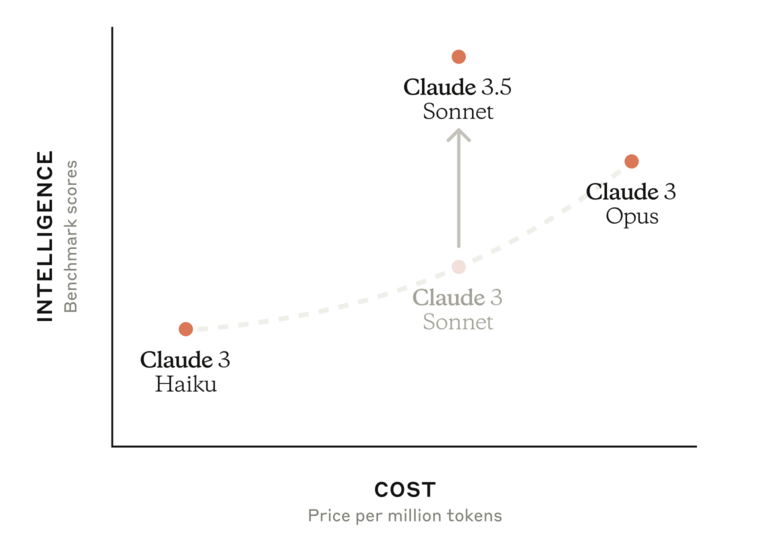
\includegraphics[width=\textwidth]{figures/3-5-sonnet-curve.png}
  \caption{Anthropic API dokumentaatiossa oleva havannollistava kuva mallien eroista 05.08.2024}
  \label{fig:3-5-sonnet-curve}
\end{figure}

Claudea on mahdollista kokeilla web-käyttöliittymän kautta rekisteröitymisen
jälkeen ilmaisena muutamia kyselyitä päivässä \parencite{claudeChat}. Tarjolla
on myös Anthropic API, joka vaatii aktiivisen tilauksen. APIa voi käyttää
tarjolla olevien kirjastojen avulla tai vaihtoehtoisesti suorittaa itse kutsuja
API-dokumentaation mukaisesti. Claude on saatavilla myös AWS Bedrockin sekä
Vertex AI:n kautta. \parencite{anthropicAPIDocs}

\subsection{Käyttö}
\label{ch:claude-usage}

Anthropic tarjoaa vain Python-kirjastoja Clauden käyttöön, joten sovellukseen
integrointi tehdään kutsuen suoraan saatavilla olevaa rajapintaa. Yksi
yksinkertainen vaihtoehto on käyttää openfeign:iä, joka saadaan käyttöön
lisäämällä `pom.xml`:n riippuvuuksiin \ref{lst:openfeign-pom.xml} mukainen
riippuvuus.

\begin{lstlisting}[
    basicstyle=\small,
    caption={spring-cloud-starter-openfeign riippuvuus pom.xml tiedostoon},
    label={lst:openfeign-pom.xml},
    language=xml,
]
<dependency>
    <groupId>org.springframework.cloud</groupId>
    <artifactId>spring-cloud-starter-openfeign</artifactId>
    <version>4.1.3</version>
</dependency>
\end{lstlisting}

Openfeign riippuvuuden lisäämisen jälkeen saadaan määritään kohdassa
\ref{lst:ClaudeConfig.java} oleva konfiguraatio, jotta saadaan jokaiseen
pyyntöön lisätty otsikkotietoihin API-avain ja versio, joita rajapinnan
käyttämisen vaatii \parencite{anthropicAPIDocsVersions}
\parencite{anthropicAPIDocsGettingStarted}.

\begin{lstlisting}[
    basicstyle=\small,
    caption={Konfiguraation Claude:lle luodulle Openfeign clientille},
    label={lst:ClaudeConfig.java},
    language=java,
]
public class ClaudeConfig {

    // Luetaan ympäristömuuttujista API avain
    @Value("${CLAUDE_API_KEY}")
    private String CLAUDE_API_KEY;

    @Bean
    public RequestInterceptor requestInterceptor(){
        // Lisätään käytettävä versio ja API avain pyyntöjen
        // otsikkotietoihin
        return requestTemplate -> {
            requestTemplate.header("anthropic-version", "2023-06-01");
            requestTemplate.header("x-api-key", CLAUDE_API_KEY);
        };
    }
}
\end{lstlisting}

Tämän jälkeen määritellään interface, josta OpenFeign luo käytettävän clientin.
Kyseinen interface on nähtävissä kohdassa \ref{lst:ClaudeApiClient.java}.

\begin{lstlisting}[
    basicstyle=\small,
    caption={Konfiguraation Claude:lle luodulle Openfeign clientille},
    label={lst:ClaudeApiClient.java},
    language=java,
]
// Kerrotaan OpenFeign:lle, että tämän interfacen perusteella tulee
// luoda toteutus Claude rajapinnalle
@FeignClient(
    name = "claude-api",
    url = "https://api.anthropic.com/v1/",
    configuration = ClaudeConfig.class
)
public interface ClaudeApiClient {

    // Määritellään mahdolliset pyynnöt

    @PostMapping("messages")
    MessagesResponse messages(@RequestBody MessagesRequest messagesRequest);
}
\end{lstlisting}

OpenFeign luo määritellyn interfacen pohjalta automaattisesti ilmiintymän, jota
voidaan käyttää kohdan \ref{lst:ClaudeService.java} mukaisesti.

\begin{lstlisting}[
    basicstyle=\small,
    caption={Konfiguraation Claude:lle luodulle Openfeign clientille},
    label={lst:ClaudeService.java},
    language=java,
]
// Merkitään luokka Serviceksi Spring Frameworkille
@Service
@RequiredArgsConstructor
public class ClaudeService {

    // OpenFeign luo automaattisesti ilmiintymän, jonka Spring
    // Framework alustaa tähän muuttujaan
    private final ClaudeApiClient claudeApiClient;

    public void example() {
        // Luodaan pyyntö
        var request = new MessagesRequest(new Message("user", "Hello world!"));
        // Tehdään pyyntö
        var response = claudeApiClient.messages(request);

        // Tässä voidaan käsitellä saatu vastaus miten halutaan
    }
}
\end{lstlisting}

\subsection{Hinnoittelu}

Clauden hinnoittelu vaihtelee hiukan sivuston mukaan. Claude.ai:n Pro-tilauksen
hinnoiksi ilmoitetaan \$20 tai 18€ + ALV ja Team-tilaukselle \$25/\$30 tai
23€/28€ + ALV. \parencite{anthropicPricing} \parencite{claudePricing} Anthropic
API:n hinnat on esitetty taulukossa \ref{tab:anthropic-api-pricing}

\begin{table}[H]
  \centering
  \rowcolors{2}{gray!25}{white}
  \caption{Anthropic APIn hinnat}
  \label{tab:anthropic-api-pricing}
  \begin{tabular}{lcc}
    \textbf{Malli} & \textbf{Syöttö} & \textbf{Ulostulo} \\
    \hline
    Claude 3.5 Sonnect &    \$3 / MTok &   \$15 / MTok \\
    Claude 3 Opus      &   \$15 / MTok &   \$75 / MTok \\
    Claude 3 Haiku     & \$0.25 / MTok & \$1.25 / MTok \\
    \hline
  \end{tabular}
\end{table}

Clauden ilmainen tilaus sisältää vain Claude 3.5 Sonnetin käyttämisen
web-käyttöliittymän sekä sovellusten kautta. Pro-tilaus lisää mahdollisuuden
käyttää Opus- ja Haiku-malleja sekä joitain QoL-lisäyksiä ja suurempaa
prioriteettia käyttäjälle. Team-tilaus on lähinnä tiimin hallinnan ja maksun
kannalta oleellisia lisätoiminnallisuuksia. Pro-tilaus lisää viisinkertaisen
käyttörajan verrattuna ilmaiseen ja Team-tilaus sitäkin suuremman.
\parencite{anthropicPricing} \parencite{claudePricing} Selviä käyttörajoja ei
ole saatavilla.

\section{xAI}

XAi on Elon Muskin johtama tekoälyritys, joka on luonut Grok-kielimallin
\parencite{xAIAbout}. Grok-kielimallin on epäilty olevan vain yksi kielimalli
lisää muiden joukossa \parencite{fireshipElonsGrokAI}, jonka perustamisen
taustalla vaikuttaa olevan ennemminkin huumoriset päähänpistokset
\parencite{twitter1679182035645235200} ja erimielisyydet ja oikeusjutut
muun muassa OpenAI:n kanssa, jonka perustajistoon Elon Musk kuuluu
\parencite{fireshipElonsLawsuitAgainstOpenAI}.

Marraskuussa 2024 Grok-kielimallille avattiin rajapinta, jota kehittäjät
pääsevät kokeilemaan vähintään vuoden 2024 loppuun asti. Jokaiselle
rekisteröityneelle annetaan ilmaista kredittiä 25 dollarin verran
kuukaudessa. Rajapinta on toteuttu yhteensopivaksi OpenAI:n ja Anthropicin
tarjoamien rajapintojen kanssa, joka mahdollistaa jo tehtyjen toteutuksien
erittäin helpon vaihtamisen käyttämään xAI:n rajapintaa. \parencite{xAIBlogApi}

\subsection{Käyttö}

Dokumentaatiossa luetellut integraatiot pohjautuvat olemassa oleviin OpenAI:n
ja Anthropic SDK:hin, jotka on toteutettu JavaScriptille ja Pythonille
\parencite{xAIDocsIntegrations}. Näiden käyttö ei tällöin onnistu suoraan
työn ohella tehdyn sovelluksen kanssa, joten toteutus tulee tehdä tarjolla
olevan REST-rajapinnan kautta, kuten luvussa \ref{ch:claude-usage} tehtiin
Clauden kanssa.

Saamme API-avaimen määriteltyä dokumentaation mukaisesti otsikkotietoihin
kohdassa \ref{lst:XAIConfig.java} esitellyllä tavalla.

\begin{lstlisting}[
    basicstyle=\small,
    caption={Konfiguraation xAI:lle luodulle Openfeign clientille},
    label={lst:XAIConfig.java},
    language=java,
]
public class XAIConfig {

    // Luetaan api avain ympäristömuuttujista
    @Value("${XAI_API_KEY:}")
    private String XAI_API_KEY;

    @Bean
    public RequestInterceptor requestInterceptor() {
        // Lisätään API-avain Authorization-otsikkotietoon
        return requestTemplate -> requestTemplate
            .header("Authorization", "Bearer " + GROK_API_KEY);
    }
}
\end{lstlisting}

Tämän jälkeen määritellään interface, josta OpenFeign luo käytettävän clientin.
Kyseinen interface on nähtävissä kohdassa \ref{lst:XAIApiClient.java}.

\begin{lstlisting}[
    basicstyle=\small,
    caption={Interface xAI:n rajapinnasta},
    label={lst:XAIApiClient.java},
    language=java,
]
// Kerrotaan OpenFeign:lle, että tämän interfacen perusteella tulee
// luoda toteutus xAI rajapinnasta
@FeignClient(
    name = "xai-api",
    url = "https://api.x.ai/v1/",
    configuration = XAIConfig.class
)
public interface XAIApiClient {

    // Määritellään mahdolliset pyynnöt

    @PostMapping("chat/completions")
    ChatCompletionsResponse chatCompletions(
        @RequestBody ChatCompletionsRequest chatCompletionsRequest
    );
}
\end{lstlisting}

OpenFeign luo määritellyn interfacen pohjalta automaattisesti ilmiintymän, jota
voidaan käyttää kohdan \ref{lst:XAIService.java} mukaisesti.

\begin{lstlisting}[
    basicstyle=\small,
    caption={Service, jossa varsinanen rajapinnan kutsuminen tapahtuu},
    label={lst:XAIService.java},
    language=java,
]
// Merkitään luokka Serviceksi Spring Frameworkille
@Service
@RequiredArgsConstructor
public class GrokService {

    // OpenFeign luo automaattisesti ilmiintymän, jonka Spring
    // Framework alustaa tähän muuttujaan
    private final GrokApiClient grokApiClient;

    public void example() {
        // Alustetaan keskustelu
        List<Message> messages = new ArrayList<>();
        messages.add(new Message("system", "Kerrot vitsejä käyttäjän antamista aiheista"));
        messages.add(new Message("user", "omena"));

        // Luodaan pyyntö keskustelun pohjalta
        ChatCompletionsRequest request =
            new ChatCompletionsRequest("grok-beta", messages);

        // Kutsutaan rajapintaa luodulla pyynnöllä
        ChatCompletionsResponse response =
            grokApiClient.chatCompletions(request);

        // Tulostetaan vastaus
        System.out.println(
            response.choices().getFirst().message().content());
    }
}
\end{lstlisting}

\subsection{Hinnoittelu}

XAI:n rajapinnan hinnoittelua ei ole avattu julkisilla sivuilla, mutta
rekisteröitymällä osaksi uuden rajapinnan julkista betaohjelmaa pääsee näkemään
eri mallien hinnoittelut ja rajoitukset. Nämä hinnat on koottu taulukkoon
\ref{tab:grok-prices} joulukuussa 2024.

\begin{table}[H]
    \centering
    \rowcolors{2}{gray!25}{white}
    \caption{xAI:n tarjomien kielimallien hinnat joulukuussa 2024}
    \label{tab:grok-prices}
    \begin{tabular}{llcc}
        \textbf{Malli} & \textbf{Syöttö (teksti)} & \textbf{Syöttö (kuva)} & \textbf{Ulostulo} \\
        \hline
        grok-beta          & \$5.00 / MTok &             - & \$15.00 / MTok \\
        grok-vision-beta   & \$5.00 / MTok & \$5.00 / MTok & \$15.00 / MTok \\
        grok-2-vision-1212 & \$2.00 / MTok & \$2.00 / MTok & \$10.00 / MTok \\
        grok-2-1212        & \$2.00 / MTok &             - & \$10.00 / MTok \\
        \hline
    \end{tabular}
\end{table}

Vastaavat tiedot malleista ja hinnoista saa haettua myös xAI:n rajapinnan
tarjoamasta päätepisteestä. \parencite{xAIDocsEndpoints}

\section{Sovellukseen valittavat kielimallit}

Aiemmin määriteltyjen ehtojen mukaisesti, on sovellukseen valittavissa
kielimalleissa ensisijaisena vaatimuksena hinnoittelu ja toisena kohtuullinen
tapa toteuttaa. Esitellyistä kielimalleista kaikki olivat mahdollista toteuttaa
kohtuullisesti, joten käytännössä vain hinta ratkaisee.

Esitellyistä kielimalleista Claude vaatii erillisen tilauksen, jotta se
voitaisiin integroida sovellukseen eikä tarjoa käytönmukaista hinnoittelua tai
vaihtoehtoisesti tarjoa kokeilujaksoa tai -krediittejä. VertexAI:n ansiosta
saadaan integroitua Gemini, PaLM 2 ja Llama käytännössä yhdellä toteutuksella,
joten ei ole syytä olla integroimatta niistä jotain kun integroidaan yksikin.
Sovellukseen tehdään tuki useille kielimalleille, jotta niitä voidaan kokeilla
varsinaisessa käytössä, joten ei ole myöskään syytä olla integroimatta xAI:ta
osaksi sovellusta. Sovellukseen valittuja kielimalleja ovat siis Gemini,
PaLM 2, Llama ja xAI. Jokaisesta kielimallista valitaan tekohetkellä
kielimallien uusin versio ja dokumentaation peruskäyttöön suosittelema
variaatio, mikäli kielimallista on useita variaatioita.


\chapter{Sovellus}
\label{ch:sovellus}

Rippikoulujen sisältö pohjautuu rippikoulusuunnitelmaan
\parencite{evlSuuriIhmeRippikoulusuunnitelma2017}, joka määrittää pääraamit
muun muassa sille kaikelle, mitä rippikoulussa käsitellään. Yksi rippikoulun
tärkeistä osaalueista on isoset ja heidän osallistumisensa ohjelman
suunnitteluun ja järjestämiseen. Rippikoulusuunnitelmassa
\parencite{evlSuuriIhmeRippikoulusuunnitelma2017} mainitaankin:

\begin{quotation}
    \noindent Isoset ovat tärkeä osa rippikoulun kokonaisuutta ja myös
    rippikoulun tiimiä. Siksi seurakunnan isostoimintaa ja rippikoulujen
    kokonaisuutta kannattaa suunnitella yhdessä. Isosilla on keskeinen rooli
    rippikoululaisten samastumiskohteina ja ”isosisaruksina”. Rippikoululaiset
    oppivat usein isosilta enemmän kuin ohjaajilta.
\end{quotation}

Rippikoulusuunnitelmassa tuodaan esille se, että eri paikkakunnilla ja eri
seurakunnilla on erilaiset mahdollisuudet järjestää asioita. Tässä työssä
tilannetta katsellaan erityisesti Ruokolahden seurakunnan isosten näkökulmasta.

Ruokolahden seurakunnalla rippikoulu koostuu muun muassa kirkkokäynneistä,
nuortenilloista, etätehtävistä, opetuspäivistä ja lopulta varsinaisesta
leiristä. Vuoden aikana isoskoulutusta käyvät isoset sekä aiempina vuosina
isoskoulutuksen käyneet osallistuvat järjestämään ohjelmaa vuoden aikana
käytäviin nuorteniltoihin sekä ovat avustamassa jumalanpalveluksissa sekä
opetuspäivissä. Nämä ovat yksittäisiä pienempiä asioita, jotka saadaan
yleensä järjestettyä pienemmällä määrällä. Varsinaisella leirillä kuitenkin
tahti on toisenlainen. Parin tunnin ohjelman sijaan leiriläisille luodaan koko
leirin ajaksi ohjelma, joka sisältää joka päivä toimintaa heräämisestä
hiljaisuuteen asti. Tähän tiiviiseen ohjelmaan pakataan kaikki asiat, joita
rippikoululla käydään läpi. Ohjelmarunko ja opetus on suunniteltu etukäteen,
mutta elää tilanteen mukaan ja harvemmin pysyy alkuperäisessä edes yhtä
kokonaista päivää. Ohjelman ollessa tiivis ja muutosten tullessa tilanteen
tarvittaessa erittäin lyhyellä varoitusajalla ja rippikoulutiimin koostuessa
yleensä noin neljästä aikuisesta, kymmenestä isosesta sekä vierailijoista,
kuten kanttorista ja diakonissasta, on tärkeää, että kaikki ovat ajantasalla
milloin mitäkin tapahtuu. Ruokolahden seurakunnalla tähän käytettiin pitkään
ensisijaisesti ja ainoana keinona yhtä WhatsApp-ryhmäkeskustelua, johon
kuuluivat lähes kaikki, jotka olivat läsnä leirillä. Leirin ollessa viikon
mittainen, oli viimeisinä päivinä viestien määrä tuhansissa ja mediaa, kuten
kuvia ja pdf:iä, useita satoja. Tällöin sisällön etsintä muuttui yhä
hankalammaksi viikkoa loppuun mennessä ja tiedotetut muutokset olivat pitkälti
muistin varassa.

Tämän työn ohessa on luotu sovellus, joka pyrkii tuomaan helpostusta edellä
kuvattuun tilanteeseen ja keventämään erityisten isosten työkuormaa, mutta
samalla myös ohjaajien. Tulevaisuudeen on mietitty myös mahdollisuutta luoda
mahdollisuus leiriläisille sekä huoltajille nähdä leiriin liittyviä asioita
sovelluksesta. Toistaiseksi sovellus on kuitenkin vain ohjaajien ja isosten
käytössä.

\section{Sovelluksen esittely}

Sovelluksesta löytyy kuvan \ref{fig:isosapp-leirit} mukaisesti kaikki leirit ja
leirien osallistujat, niin ohjaajat, isoset kuin leiriläisetkin. Leirillä
leiriläiset jaetaan leirillä isosryhmiin, jotka saadaan näkyviin leirin
päänäkymään kuvassa \ref{fig:isosapp-ryhmat}.

\begin{figure}[h!]
    \centering
    \begin{minipage}[b]{.3\textwidth}
        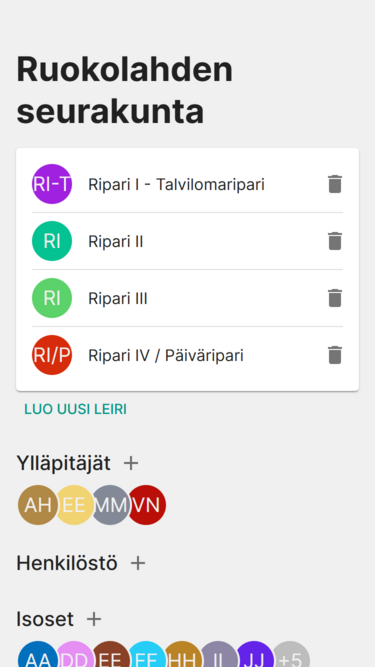
\includegraphics[width=\textwidth]{figures/isosapp-leirit.png}
        \caption{Seurakunnan näkymä, joka sisältää leirit, ohjaajat ja isoset}
        \label{fig:isosapp-leirit}
    \end{minipage}\qquad
    \begin{minipage}[b]{.3\textwidth}
        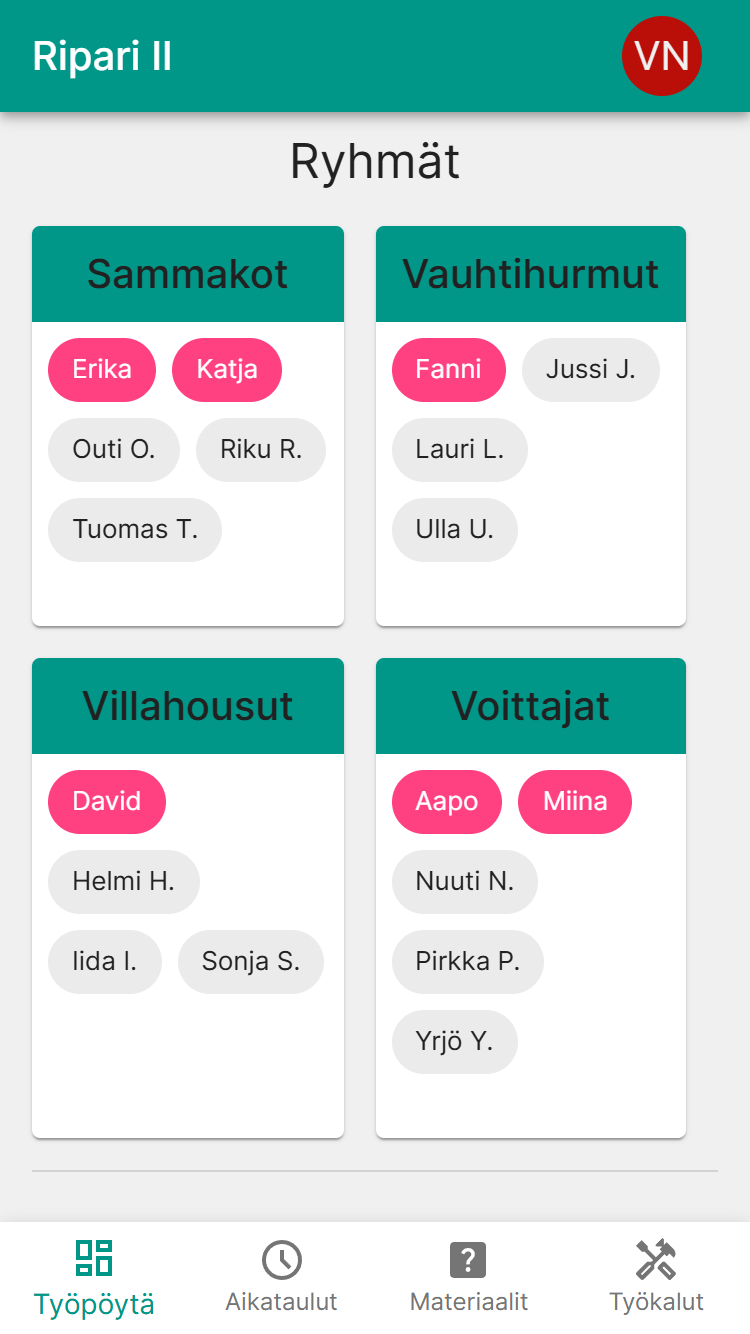
\includegraphics[width=\textwidth]{figures/isosapp-ryhmat.png}
        \caption{Leirin päänäkymän ryhmä-osio}
        \label{fig:isosapp-ryhmat}
    \end{minipage}
\end{figure}

Sovellus pohjautuu ensisijaisesti aikatauluun, jonka ympärille kaikki muu
leiriin liittyvä toiminnallisuus on rakennettu. Leirin päänäkymässä kuvassa
\ref{fig:isosapp-nakkilista} on jokaiselle näkyvissä henkilökohtainen
tehtävälista, joka näyttää seuraavan 24 tunnin sisällä olevat ohjelmat, joissa
on vetovastuuna. Samassa näkymässä on myös niin sanottu nakkilista, joka
sisältää päivittäin vaihtuvat roolit isosille. Varsinainen aikataulu löytyy
omasta näkymästä, joka on nähtävissä kuvassa \ref{fig:isosapp-aikataulu}.

\begin{figure}[h!]
    \centering
    \begin{minipage}[b]{.3\textwidth}
        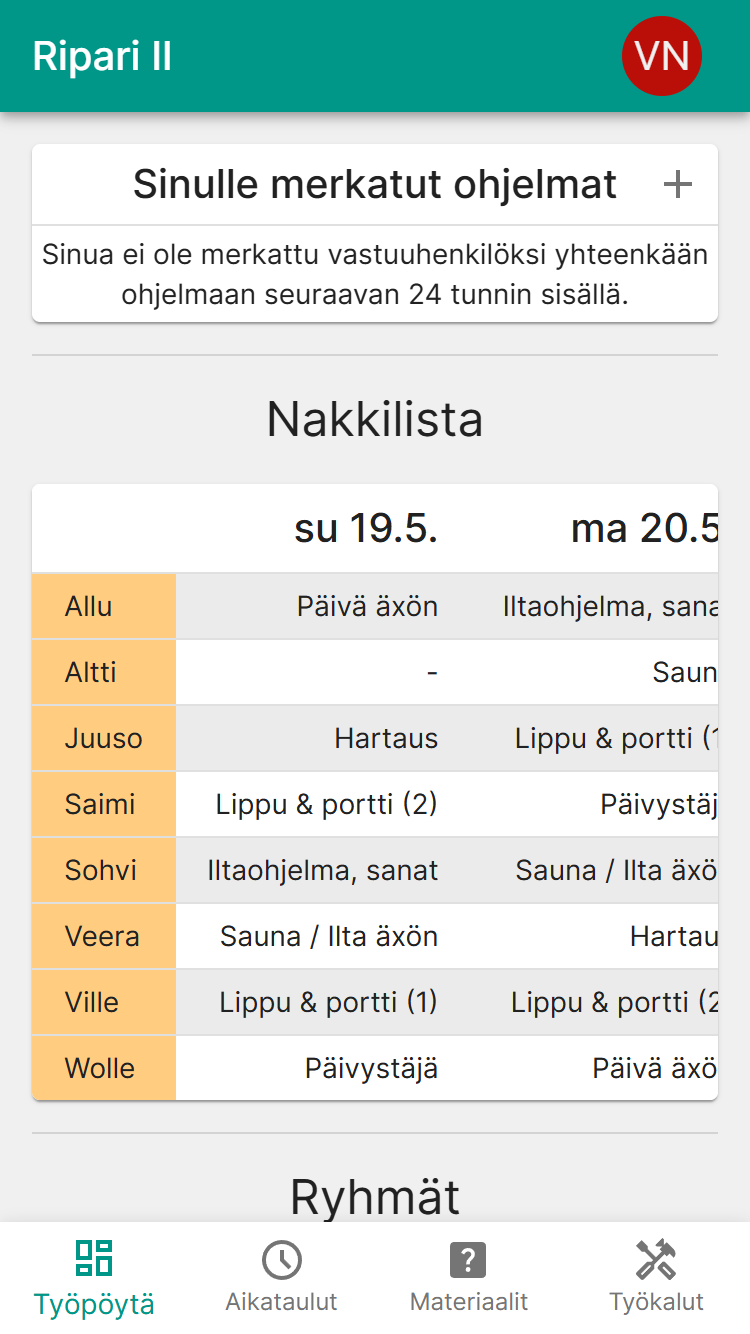
\includegraphics[width=\textwidth]{figures/isosapp-nakkilista.png}
        \caption{Leirin nakkilista ja henkilökohtainen tehtävälista}
        \label{fig:isosapp-nakkilista}
    \end{minipage}\qquad
    \begin{minipage}[b]{.3\textwidth}
        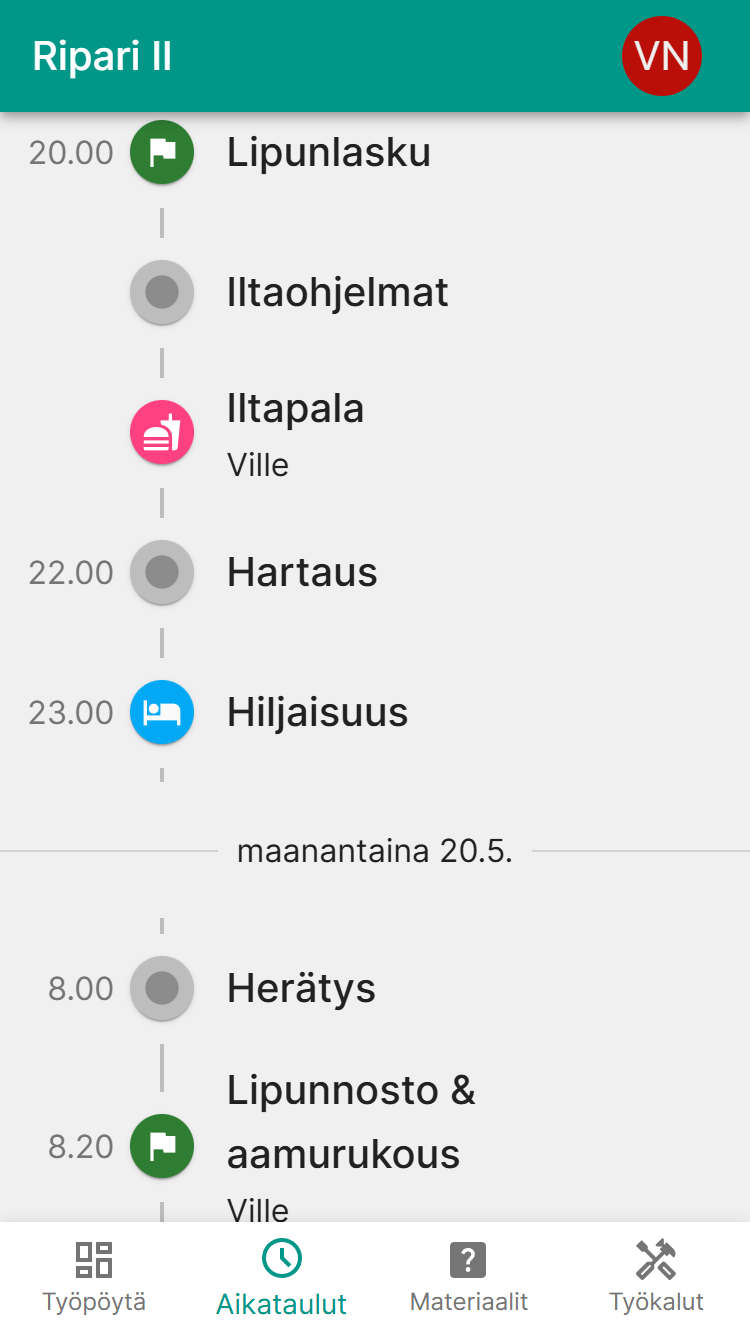
\includegraphics[width=\textwidth]{figures/isosapp-aikataulu.png}
        \caption{Leirin aikataulu ja ohjelmien vastuuhenkilöt}
        \label{fig:isosapp-aikataulu}
    \end{minipage}
\end{figure}

Näiden lisäksi ohjelman suunnittelua helpottamaan on luotu materiaalipankki,
josta löytyy kisoja, leikkejä ja sketsejä sekä listoja lauluista. Aikataulussa
oleviin ohjelmat on mahdollista linkittää suoraan materiaaliin, joten
ohjelmasta pääsee helposti näkemään mm. kilpailun säännöt, kuten kuvassa
\ref{fig:isosapp-materiaalit}. Materiaalin lisäksi ohjelman tekemisessä
tarvitaan välillä yksinkertaisia työkalua, kuten ryhmien arvontaa tai
telepromteria leikkimielisten uutisten lukemiseen. Näitä varten on luotu
kuvassa \ref{fig:isosapp-tyokalut} näkymä työkalu näkymä.

\begin{figure}[h!]
    \centering
    \begin{minipage}[b]{.3\textwidth}
        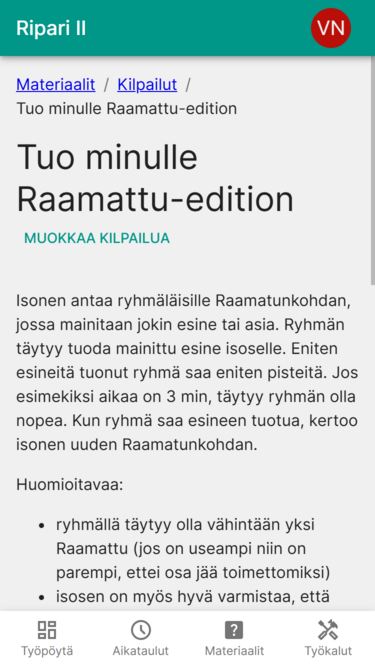
\includegraphics[width=\textwidth]{figures/isosapp-materiaalit.png}
        \caption{Esimerkki materiaaleihin lisätystä kilpailusta}
        \label{fig:isosapp-materiaalit}
    \end{minipage}\qquad
    \begin{minipage}[b]{.3\textwidth}
        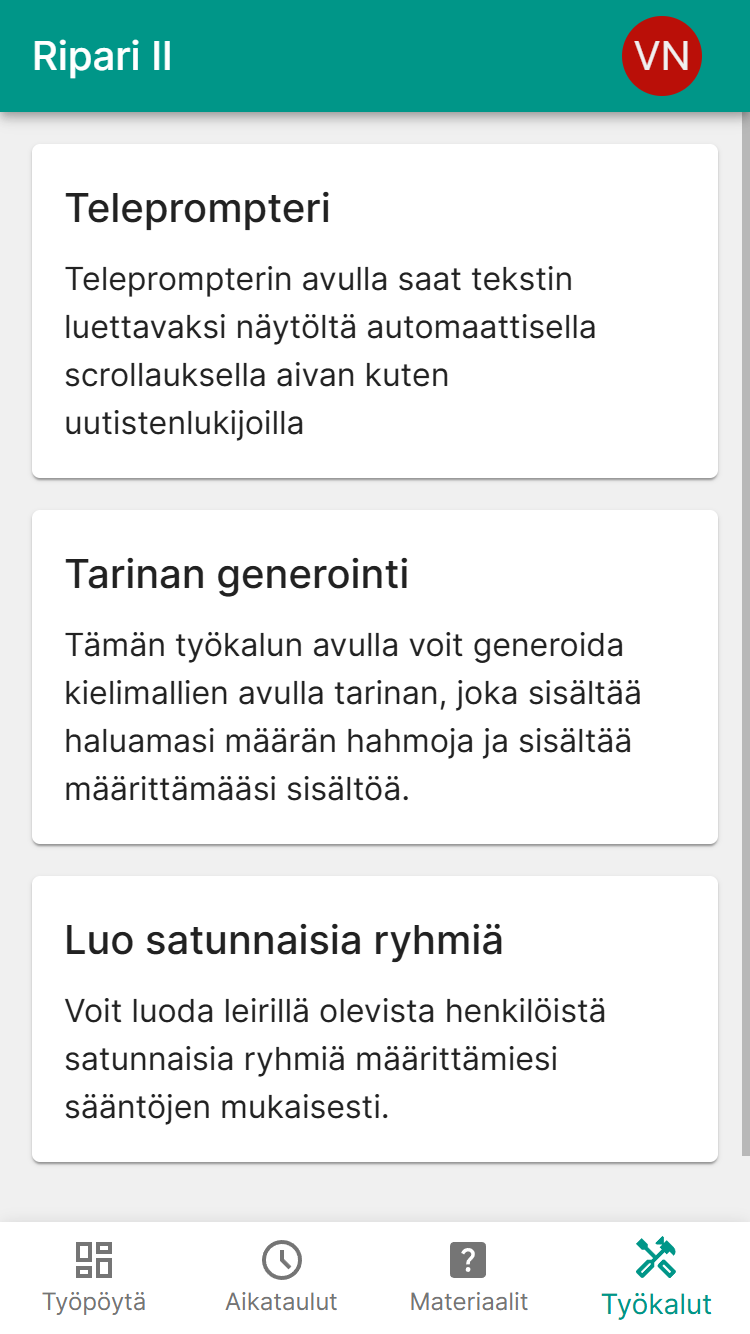
\includegraphics[width=\textwidth]{figures/isosapp-tyokalut.png}
        \caption{Sovelluksen työkalu-näkymä}
        \label{fig:isosapp-tyokalut}
    \end{minipage}
\end{figure}

\clearpage
\section{Kielimallien integrointi osaksi sovellusta}

\begin{wrapfigure}{r}{0.45\textwidth}
    \centering
    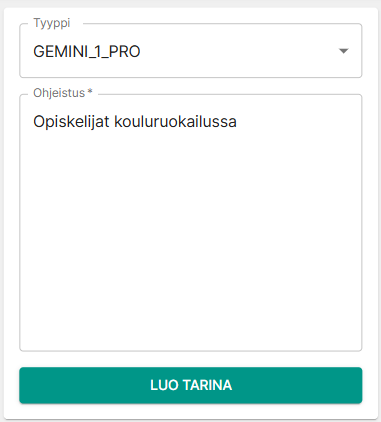
\includegraphics[width=0.45\textwidth]{figures/isosapp-tyokalut-tarinan-generointi-1.png}
    \caption{Tarinan luontinäkymä}
    \label{fig:isosapp-tyokalut-tarinan-generointi-1}

    \qquad

    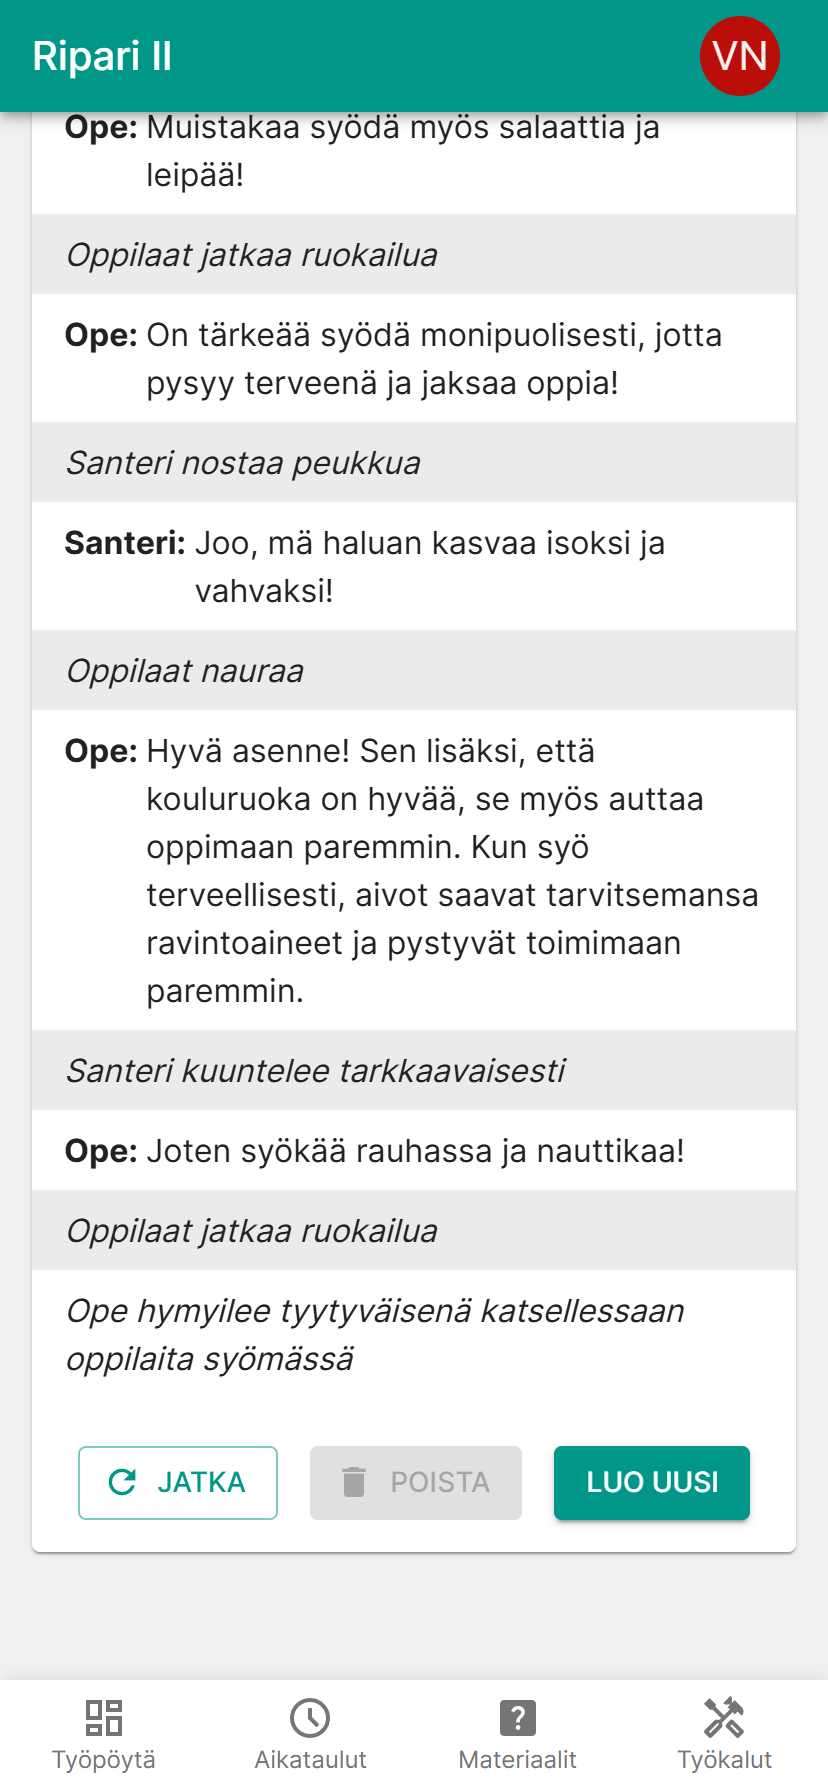
\includegraphics[width=0.45\textwidth]{figures/isosapp-tyokalut-tarinan-generointi-2.png}
    \caption{Sovelluksen työkalu-näkymä}
    \label{fig:isosapp-tyokalut-tarinan-generointi-2}
\end{wrapfigure}

Kielimallit ovat hyviä tuottamaan paljon sisältöä ja nopeasti. On tilanteita,
joissa tällaisesta on hyötyä, vaikka sisältöä ei olisikaan laadullisesti
parasta mahdollista. Yhtenä esimerkkinä tästä on työkalu, jolla saa generoitua
tarinaa. Tätä tarinaa voidaan käyttää pohjana muun muassa sketsien luomisessa.

Sovellukseen on toteutettu kielimalleja hyödyntävä työkalu, jolle saa valittua
käytettävän kielimallin ja annettua ohjeistuksen, mitä tarinan tulisi sisältää,
kuvan \ref{fig:isosapp-tyokalut-tarinan-generointi-1} mukaisesti.
Käyttöliittymä osaa näyttää tarinan vuorosanat sekä toiminnot, kuten kuvassa
\ref{fig:isosapp-tyokalut-tarinan-generointi-2} nähdään. Käyttöliittymä tukee
myös tarinan jatkamista mikäli vain valittulle kielimmallille on toteutettu
kyseinen toiminnallisuus taustajärjestelmän puolelle.

Työkalun lähtökohtana ollut päästä testaamaan useampaa eri kielimallia, joten
toteutuksesta on pyritty tekemään mahdollisimman joustava useammalla eri
kielimallille. Jokaisen kielimallin toteutuksen tulee toteuttaa
\ref{lst:StoryLineService.java} interfacen kaikki metodit, jotta kielimallia
saadaan käytettyä olemassa olevan käyttöliittymän kanssa. Metodit heittävät
poikkeuksen, mikäli suoritus ei onnistunut, jolloin käyttöliittymä näyttää
virheen ja mahdollistaa uudelleen yrittämisen.

\clearpage
\begin{lstlisting}[
    basicstyle=\small,
    caption={StoryLineService interface, jonka toteuttamalla kielimallit saadaan },
    label={lst:StoryLineService.java},
    language=java,
]
public interface StoryLineService {

    List<StoryLine> createStoryLines(Story story);
    List<StoryLine> continueStoryLines(Story story);
    void cleanUp(Story story);
}
\end{lstlisting}

\subsection{Gemini toteutus}

Aiemmin kohdassa \ref{lst:GeminiServiceExample.java} esitelty GeminiService
saadaan käyttöön toteuttamalla StorylineService-interfacessa määritellyt
metodit tarinan luomiselle ja jatkamiselle esimerkin
\ref{lst:GeminiService.java} mukaisesti. Geminin kanssa on mahdollista käyttää
ChatSessionia, joka mahdollistaa viestien lähettämisen edestakaisin niin, että
kielimallilla on suoraan käytettävissä aiempi viestittely kontekstina. Tämän
ansiosta tarinaa on helppo jatkaa kunhan aiemmin luotu ChatSession on yhä
käytettävissä.

\begin{lstlisting}[
    basicstyle=\small,
    caption={Esimerkki GeminiServicen StorylineService-interfacen vaatimien metodien toteutuksesta},
    label={lst:GeminiService.java},
    language=java,
]
// Map, johon voidaan tallentaa luodut ChatSessionit myöhempää
// käyttöä varten
private final Map<UUID, ChatSession> chatSessions =
    new ConcurrentHashMap<>();

@Override
public List<StoryLine> createStoryLines(Story story) {
    // Luodaan ilmiintymä mallista ja avataan ChatSession
    GenerativeModel model = new GenerativeModel(
        story.getModelName().getName(),
        vertexAI
    );
    ChatSession chatSession = model.startChat();
    chatSession.withGenerationConfig(createGenerationConfig());

    // Tallennetaan ChatSession ConcurrentHashMap:iin, jotta tarinaa
    // saadaan jatkettua tarvittaessa helposti.
    chatSessions.put(story.getId(), chatSession);

    // Pyydetään luomaan tarina
    GenerateContentResponse response =
        chatSession.sendMessage(createInitializeContent(story));

    // Käsitellään vastaus
    return parseResponse(response);
}

@Override
public List<StoryLine> continueStoryLines(Story story) {
    // Tarkistetaan onko luotua tarinaa mahdollista jatkaa
    if (!chatSessions.containsKey(story.getId()))
        throw new GoneException();

    // Haetaan olemassa oleva ChatSession
    ChatSession chatSession = chatSessions.get(story.getId());

    // Pyydetään jatkamaan tarinaa
    GenerateContentResponse response =
        chatSession.sendMessage("Jatka tarinaa");

    // Käsitellään vastaus
    return parseResponse(response);
}

@Override
public void cleanUp(Story story) {
    // Poistetaan tallessa oleva ChatSession
    chatSessions.remove(story.getId());
}
\end{lstlisting}

Tarinan alustuksessa on annettu kielimallille sanallinen ohjeistus kohdan
\ref{lst:GeminiService.java::createInitializeContent} ja liitteen
\ref{ch:gemini-guide} mukaisesti, jossa on määritelty, missä muodossa vastaus
halutaan ja mitä vastauksen pitäisi sisältää. Ohjeistukseen on liitetty
käyttäjän antama syöte käyttöliittymästä.

\begin{lstlisting}[
    basicstyle=\small,
    caption={Geminin ohjeistuksen luominen},
    label={lst:GeminiService.java::createInitializeContent},
    language=java,
]
private Content createInitializeContent(Story story) {
    String guide = "..."; // Liittestä löytyvä ohjeistus

    // Yhdistetään käyttäjän antama kuvaus ja ohjeistus tulosteesta
    return ContentMaker.fromString(story.getText() + "\n\n" + guide);
}
\end{lstlisting}

Gemini osaa tuottaa sanallisen ohjeistuksen mukaisesti vastauksen suoraan JSON-
muodossa, jolloin se pystytään parsimaan ilman, että vastausta tarvitsee
käsitellä sen enempää. Vastauksen parsiminen saadaan siis toteutettu hyvinkin
yksinkertaisesti esimerkin \ref{lst:GeminiService.java::parseResponse}
mukaisesti.

\begin{lstlisting}[
    basicstyle=\small,
    caption={Geminin vastausten käsittely},
    label={lst:GeminiService.java::parseResponse},
    language=java,
]
private List<StoryLine> parseResponse(GenerateContentResponse response)
    throws JsonProcessingException
{
    // Luetaan vastauksen teksti
    String text = response.getCandidates(0)
        .getContent()
        .getParts(0)
        .getText();

    // Parsitaan luettu json-teksti listaksi StoryLine-ilmiintymiä
    return objectMapper.readValue(text, new TypeReference<>() {});
}
\end{lstlisting}

Toteutuksen jälkeen kielimallia voidaan käyttää tuottamaan kuvassa
\ref{fig:isosapp-tyokalut-tarinan-generointi-2} näkyvä tarina kuvan
\ref{fig:isosapp-tyokalut-tarinan-generointi-1} käyttöliittymän
toiminnallisuudella.

\subsection{PaLM2 toteutus}

Vastaavasti \ref{lst:PaLM2Service.java} kohdassa esitelty PaLM2Service saadaan
toteuttamaan StorylineService-interface esimerkin
\ref{lst:PaLM2Service.java::createStoryLines} mukaisesti. PaLM 2:lle ei ole
tarjolla vastaavaa ChatSessionia, kuin Geminille, joten on sille toteutettu
vain tarinan luonti, muttei mahdollisuutta jatkaa tarinaa.

\begin{lstlisting}[
    basicstyle=\small,
    caption={Esimerkki PaLM2Servicen StorylineService-interfacen metodien toteutuksesta},
    label={lst:PaLM2Service.java::createStoryLines},
    language=java,
]
@Override
public List<StoryLine> createStoryLines(Story story) {
    // Tehdään pyyntö kielimallille
    PredictResponse predictResponse = vertexAI
        .getPredictionServiceClient()
        .predict(PredictRequest.newBuilder()
            .setEndpoint(
                getEndpointName(story.getModelName().getName())
                .toString())
            .addInstances(getPrompt(generatePrompt(story)))
            .setParameters(getParameters())
            .build());

    // Käsitellään vastaus
    return parseResponse(response);
}
\end{lstlisting}

PaLM2-kielimallille on luotu vastaava ohjeistuis kuin Geminille, jossa
määritellään minkälainen vastaus kielimallin tulisi tuottaa ja kielimallille
annetaan käyttäjän antama syöte. Ohjeistuksen toteutus on nähtävissä kohdassa
\ref{lst:PaLM2Service.java::generatePrompt} ja koko ohjeistus liitteessä \ref{ch:palm2-guide}.

\begin{lstlisting}[
    basicstyle=\small,
    caption={PaLM2 ohjeistuksen luonti},
    label={lst:PaLM2Service.java::generatePrompt},
    language=java,
]
private String generatePrompt(Story story) {
    String guide = "..."; // Liitteestä löytyvä ohjeistus

    // Yhdistetään käyttäjän antama syöte ja ohjeistus
    return story.getText() + "\n\n" + guide;
}

// Apufunktio ohjeistuksen muuttamiseen kielimallin haluamaan muotoon
private com.google.protobuf.Value getPrompt(String prompt) throws
    InvalidProtocolBufferException, JsonProcessingException
{
    Map<String, Object> instance = new HashMap<>();
    instance.put("prompt", prompt);
    return convertMapToValue(instance);
}
\end{lstlisting}

PaLM2:sta ohjeistaessa sanallisesti, että tuloksen tulee olla JSON-muodossa,
tulee tuloste Markdownin tukemassa JSON-muodossa, jossa varsinanen JSON osuus
on ympäritöity JSON-koodiosiota tarkoittavilla merkinnöillä. Jotta tulos
saadaan käsitelty, tulee vastauksesta saada nämä pois. Tämä saadaan toteutettua
esimerkin \ref{lst:PaLM2Service.java::parseResponse} mukaisesti.

\begin{lstlisting}[
    basicstyle=\small,
    caption={PaLM2 vastauksen käsittely},
    label={lst:PaLM2Service.java::parseResponse},
    language=java,
]
private List<StoryLine> parseResponse(PredictResponse response)
    throws JsonProcessingException
{
    String json = response
        .getPredictions(0)
        .getStructValue()
        .getFieldsOrThrow("content")
        .getStringValue()
        .replaceFirst("```json\n", "")
        .replaceFirst("```", "");

    return objectMapper.readValue(json, new TypeReference<>() {});
}
\end{lstlisting}

\subsection{Llama 3 toteutus}

Kun Llama 3:sta käytetään VertexAI:n tarjoaman kirjaston kautta, tukee se
samoja toimintoja, kuin mitä on käytetty Geminin toteutuksessa. Toteutus
saadaan tällöin tehtyä samanlaisena kuin Geminillä kohdassa
\ref{lst:GeminiService.java}.

Kielimallille annettava ohjeistus eroaa kuitenkin siitä, mitä Geminille
annetaan. Ohjeistus saadaan luotua vastaavasti kuin Geminille kohdassa
\ref{lst:GeminiService.java::createInitializeContent}, mutta ohjeistuksena
annettava teksti on liitteessä \ref{ch:llama3-guide}. Ohjeistus on vastaava
kuin PaLM2:lla, mutta kielimallille tuli erikseen sanoa, että tulosteessa ei
saa olla muuta kuin JSON-vastaus, jotta kielimalli jätti ylimääräisen
tulosteen pois ja tuotti vain halutun tuloksen.

\subsection{xAI:n toteutus}

XAI:n rajapinnan dokumentaatiossa on määritelty 'response\_format'-kenttä, mutta
kyseiselle kentälle ei ole määritelty tyyppiä \parencite{xAIDocsEndpoints}.
Mahdollinen formaatti kyseiselle kentälle löydetään Githubissa olevasta
issuesta \parencite{githubBerriAIlitellmIssues6610}, jossa ongelmana on se,
ettei vastauksen formatointi ole tuettu sillä hetkellä. Testaamalla samalla
formaatilla saamme itsekkin vastauksena kohdassa \ref{lst:xai-bad-request.json}
näkyvän virheviestin ettei ainakaan kyseinen formatointi ole käytössä.

\begin{lstlisting}[
    basicstyle=\small,
    caption={XAI rajapinnan palauttama vastaus, kun yritetään määrittää 'response\_format'-kenttä},
    label={lst:xai-bad-request.json},
]
{
    "code":"Client specified an invalid argument",
    "error":"The model does not support formatted output but some
      have been specified in the request."
}
\end{lstlisting}

Vaikkei rajapinta suoraan vaikuta tukevan vastauksen muotoilua, voidaan ohjeet
muotoiluun antaa kirjallisesti. Alustamalla keskustelu system-roolilta
tulevalla viestillä:

\begin{quotation}
    \noindent Olet käsikirjoittaja. Luot tarinan käyttäjän antaman syötteen
    perusteella.

    \noindent Vastauksesi tulee olla JSON-muodossa oleva lista, joka koostuu
    olioista, joilla on kolme attribuuttia: type, target ja content. Type voi
    olla joko `ACTION` tai `TALK` riippuen siitä, onko kyseessä jotakin mitä
    tapahtuu vai jotain mitä joku sanoo. Target kuvastaa sitä kuka tekee tai
    kuka sanoo. Content kuvastaa sitä mitä tapahtuu tai sanotaan.
\end{quotation}

saadaan vastaukset halutussa JSON-muodossa, jonka myötä saadaan viesti
parsittua StoryLineService-interfacen metodien vastauksien haluamaan
muotoon antamalla vastaus suoraan JSON-parserille kohdan
\ref{lst:XAIService.java::parseResponse} mukaisesti.

\begin{lstlisting}[
    basicstyle=\small,
    caption={XAI rajapinnan palauttaman vastauksen parsiminen haluttuun muotoon},
    label={lst:XAIService.java::parseResponse},
    language=java,
]
private List<StoryLine> parseResponse(Message message)
    throws IOException
{
    // Luetaan viestin sisältö ja poistetaan ylimääräinen muotoilu
    String json = message.content()
        .replaceFirst("```json\n", "")
        .replaceFirst("```", "");

    // Luetaan tekstimuodossa oleva json listaksi StoryLine-olioita
    return objectMapper.readValue(json, new TypeReference<>() {});
}
\end{lstlisting}

Käytettävä rajapinta päätepiste pohjautuu alunperinkin siihen, että sinne
lähetetään lista viesteistä. Tätä hyödyntämällä pystymme toteuttamaan
toiminnallisuuden tarinan jatkamiseen. Pitämällä kirjaa aiemmista viesteistä
voimme tarinan jatkamisessa yksinkertaisesti hakea vanhat viestit ja pyytää
jatkamaan tarinaa kuten kohdassa \ref{lst:XAIService.java::continueStoryLines}
olevassa toteutuksessa on tehty.

\begin{lstlisting}[
    basicstyle=\small,
    caption={XAI rajapinnan palauttaman vastauksen parsiminen haluttuun muotoon},
    label={lst:XAIService.java::continueStoryLines},
    language=java,
]
public List<StoryLine> continueStoryLines(Story story) {
    // Haetaan keskustelun vanhat viestit
    List<Message> messages = chats.get(story.getId());

    // Tarkistetaan ettei tarina kasva liian pitkäksi
    if (story.getLines().size() > 50 || messages.size() > 10)
        throw new BadRequestException("Tarina on liian pitkä!");

    // Lisätään käyttäjän pyyntö jatkaa tarinaa
    messages.add(new Message("user", "Jatka tarinaa"));

    // tehdään pyyntö
    // parsitaan vastaus
    // palautetaan uudet rivit
}
\end{lstlisting}

\section{Kielimallien toimivuuden arviointia}

Lopputuloksen ollessa tarina, jota mahdollisesti voidaan hyödyntää
ohjelmanumeroiden kehittämisessä, on sen varsinaisen tulosteen laadun arviointi
hankalaa. Työ on kuitenkin keskittynyt enemmän siihen, miten yksinkertaisesti,
helposti, nopeasti ja edullisesti saadaan toteutettua haluttu toiminnallisuus
ilman ylimääräistä työtä ja hienosäätöä. Tällöin arvioinnin kannalta oleellista
onkin se, että toimiko ratkaisu ylipäätänsä jotenkin.

Vuoden 2025 alkupuolella sovellukseen integroiduista kielimalleista ainoastaan
Gemini ja Llama3 olivat enää toiminnassa, joten toimivuuden arvioinnissa
käytettiin vain näitä kielimalleja. Suurin syy muiden kielimallien
toimimattomuuden oli rajapintojen kielteiset vastaukset puuttuvien krediittien
takia.

Arvointi toteutettiin yksinkertaisella testillä, jossa luotiin kuusi syötettä,
jotka annettiin jokaiselle kielimallille 5 kertaa ja yritettiin jokaisella
kerralla jatkaa tarinaa 5 kertaa. Annettuja syötteitä olivat seuraavat:

\begin{quotation}
    \noindent Kerro tarina opiskelijoista kouluruokailussa

    \noindent Kerro tarina kavereista matkalla elokuviin

    \noindent Kerro tarina opiskelijabileistä

    \noindent Kerro tarina työkavereista viettämässä pikkujouluja

    \noindent Kerro tarina jalkapallojoukkueesta matkalla kisoihin

    \noindent Kerro tarina leiriläisistä riparilla
\end{quotation}

Onnistuneet tarinan generoinnin määrät ovat nähtävissä graaffissa
\ref{chart:story-start}. Onnistumiseksi laskettiin se, että tarinaan saatiin
tuotettuja rivejä, kun puolestaan epäonnistumiseksi se, että käyttöliittymä
näytti virheilmoituksen. Teoriassa käyttöliittymä voisi näyttää muitakin
virhetilanteita kuin kielimallien integraatiossa tapahtuvia virheitä, kuten
verkko-ongelmista, mutta testin aikana tällaisia virheitä ei havaittu.

\begin{figure}[H]
    \centering
    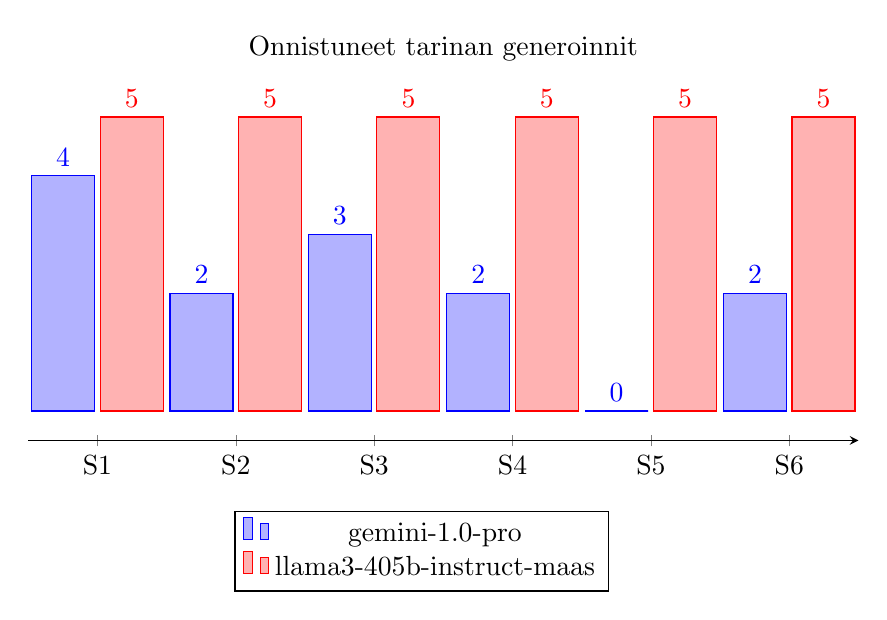
\begin{tikzpicture}
        \begin{axis}[
            ybar,
            bar width=0.8cm,
            width=\textwidth,
            height=.5\textwidth,
            title={Onnistuneet tarinan generoinnit},
            symbolic x coords={S1, S2, S3, S4, S5, S6},
            legend style={at={(0.7,-0.2)}},
            axis y line=none,
            axis x line=bottom,
            nodes near coords,
            enlargelimits=0.1,
            xtick=data,
            enlarge x limits=auto,
        ]
        \addplot+ coordinates {(S1, 4) (S2, 2) (S3, 3) (S4, 2) (S5, 0) (S6, 2)};
        \addplot+ coordinates {(S1, 5) (S2, 5) (S3, 5) (S4, 5) (S5, 5) (S6, 5)};
        \legend{gemini-1.0-pro,llama3-405b-instruct-maas}
        \end{axis}
    \end{tikzpicture}
    \caption{Onnistuneiden tarinan generointien määrät annettua syötettä kohden}
    \label{chart:story-start}
\end{figure}

Taulukon \ref{chart:story-start} tuloksista huomataan, että Llama3 onnistui
joka kerta generoimaan tarinan kun Geminin onnistuminen vaihteli huomattavasti.
Järjestelmän logien karkean läpikäynti paljasta pääasialliseksi ongelmaksi
Geminin kanssa sen, että syötteessä oli jotain muuta kuin haluttu JSON-
muotoinen vastaus. Osan kerroista pyyntö oli markdowia, osan puolestaan katkesi
kesken kaiken. Molemmat ovat tilanteita, jotka olisi mahdollista korjata melko
yksinkertaisesti tuloksen käsittelyyn, jolloin Gemini voisi päästä lähelle tai
jopa täysin samoihin tuloksiin kuin Llama3.

Sekä Gemini, että Llama3 tukivat molemmat tarinan jatkamista, joten tarinoita
yritettiin jatkaa tarinan luonnin jälkeen 5 kertaa. Näistä laskettiin
onnistuneet kerrat. Mikäli tarinan luonti epäonnistui jo alunperin, tarkoitti
se tarinan jatkamisen kannalta suoraan sitä, että tarinan jatkaminen onnistui
0 kertaa. Käyttöliittymä mahdollista virheen jälkeen sen, että tarinaa
yritettäisiin yhä jatkaa. Tätä ei kuitenkaan tehty sillä kielimallin kanssa
käyty keskustelu sisälsi tällöin virhetilanteessakin luodun osan, joka ei
näkynyt käyttäjälle, mutta oli kielimallille tiedossa, joten tarinan
yhtenäisyys kärsi jokaisesta virheestä. Määrät onnistuneista tarinan
jatkamisista ovat nähtävissä graaffissa \ref{chart:story-continue}. Tarinan
jatkamisessa Geminin kohdanneet ongelmat olivat vastaavia kuin tarinan
luonnissa.

\begin{figure}[H]
    \centering
    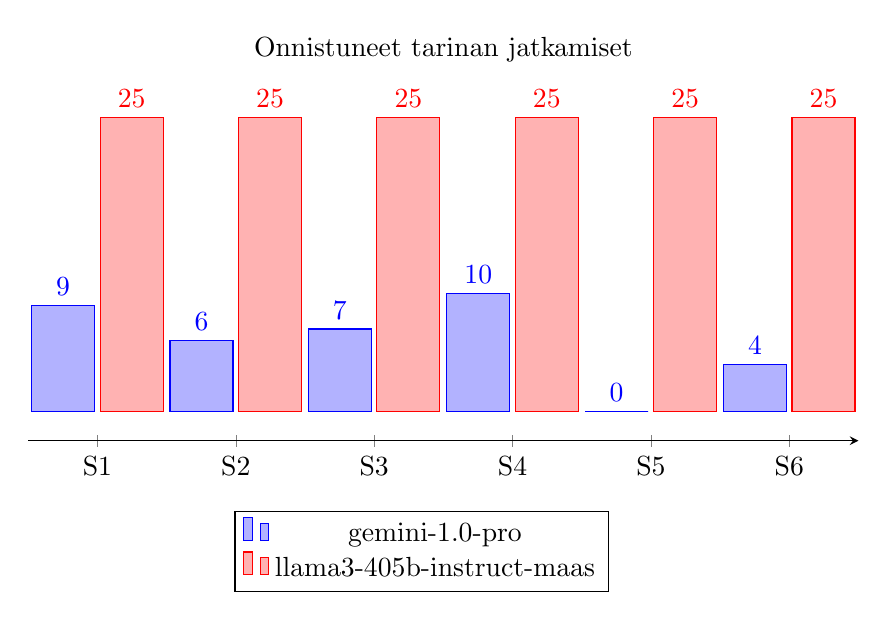
\begin{tikzpicture}
        \begin{axis}[
            ybar,
            bar width=0.8cm,
            width=\textwidth,
            height=.5\textwidth,
            title={Onnistuneet tarinan jatkamiset},
            symbolic x coords={S1, S2, S3, S4, S5, S6},
            legend style={at={(0.7,-0.2)}},
            axis y line=none,
            axis x line=bottom,
            nodes near coords,
            xtick=data,
            enlarge x limits=auto,
        ]
        \addplot+ coordinates {(S1, 9) (S2, 6) (S3, 7) (S4, 10) (S5, 0) (S6, 4)};
        \addplot+ coordinates {(S1, 25) (S2, 25) (S3, 25) (S4, 25) (S5, 25) (S6, 25)};
        \legend{gemini-1.0-pro,llama3-405b-instruct-maas}
        \end{axis}
    \end{tikzpicture}
    \caption{Onnistuneiden tarinan jatkamisien määrät aiemmin annettujen syötteiden pohjalta luoduille tarinoille}
    \label{chart:story-continue}
\end{figure}

Jokaiselle onnistuneelle tarinan generoinnille laskettiin rivimäärä, joka
sisältää sekä vuorosanat että toiminnan. Graaffista \ref{chart:story-lines} on
nähtävissä keskimääräiset määrät tuotetuille riveille.

\begin{figure}[H]
    \centering
    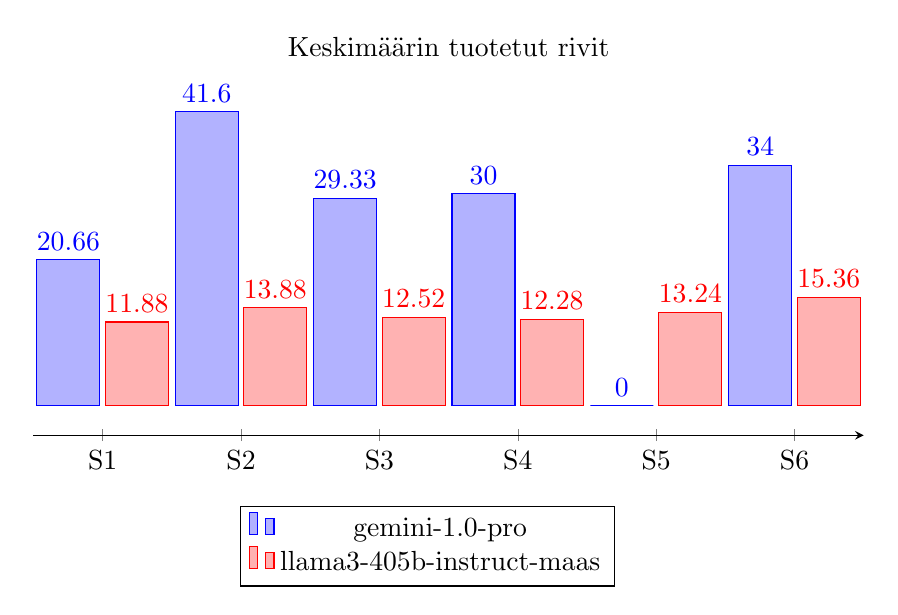
\begin{tikzpicture}
        \begin{axis}[
            ybar,
            bar width=0.8cm,
            width=\textwidth,
            height=.5\textwidth,
            title={Keskimäärin tuotetut rivit},
            symbolic x coords={S1, S2, S3, S4, S5, S6},
            legend style={at={(0.7,-0.2)}},
            axis y line=none,
            axis x line=bottom,
            nodes near coords,
            xtick=data,
            enlarge x limits=auto,
        ]
        \addplot+ coordinates {(S1, 20.66) (S2, 41.6) (S3, 29.33) (S4, 30) (S5, 0) (S6, 34)};
        \addplot+ coordinates {(S1, 11.88) (S2, 13.88) (S3, 12.52) (S4, 12.28) (S5, 13.24) (S6, 15.36)};
        \legend{gemini-1.0-pro,llama3-405b-instruct-maas}
        \end{axis}
    \end{tikzpicture}
    \caption{Keskimäärin tuotettujen rivien määrä onnistuneissa pyynnöissä}
    \label{chart:story-lines}
\end{figure}

Testien tuloksien pohjalta Llama3 vaikutti suorituvan tasaisen varmasti tarinan
generoinnista, mutta Gemini puolestaan sai tuotettua enemmän tarinaa yhdellä
kertaa. Testaamisen yhteydessä lisäksi Llama3 toimi erittäin hitaasti
verrattuna Gemininiin. Tätä ei kuitenkaan mitattu vaan pohjautuu puhtaasti
testin tekijän käsitykseen tilanteesta. Geminin toimintaa testattiin myös lähes
vuosi aiemmin isosten toimesta sovellusken julkaisuhetkellä. Tuolloin isoset
eivät tuoneet esille läheskään yhtä isoa määrää virhetilanteita kuin mitä
varsinaisessa testissä tuli. Tällöin kuitenkin lähinnä keskityttiin yleiseen
mielipiteeseen ja isoimpiin puutteisiin sekä ohjelmistovirheisiin joita tuli
esille sovelluksessa itsessään, eikä tuolta ajalta ole statistiikkaa, jota
voisi verrata tuoreempiin mittauksiin.

Mittaustulosten käsittelyhetkellä Geministä oli saatavilla huomattavasti
uudempi ja kyvykkäämpi malli, joka olisi voinut olla mahdollisesti
tasapuolisempi vertailuun Llama3:n isoimman mallin kanssa. \parencite{gemini2}


\chapter{Yhteenveto}
\label{ch:yhteenveto}

Tässä työssä kokeiltiin miten eri yleisiä kielimalleja saadaan integroitua
osaksi sovellusta ilman merkittävää työmäärää tai hienosäätöä. Työssä ei
pyritty käyttämään mitään edistynyttä arviointi kriteeristöä toteutuksen
onnistumisessa tai toimivuudessa vaan hyvinkin yksinkertaisesti perus
ohjelmointitaidot omaavan harrastelijan näkökulmasta arviointia toimivuudesta.

Kielimalleja on tänä päivänä lukuisia ja jatkuvasti tulee uusia. Arviolta
puolet tässä työssä esitellyistä malleista on sellaisia, joita ei ollut vielä
olemassa työn aloitushetkellä. Kaiken kattavaa arviointia ja kokeilua onkin
mahdotonta tehdä, mutta työn pohjalta huomattiin, että usealla kielimallilla
on mahdollsita toteuttaa yksinkertaisesti totetus, joka saatii tekemään sitä
mitä haluttiin.

Jotta kielimalleille saataisiin selviä eroa, olisi yksinkertaiset virheet
korjattava ja tämän jälkeen luotava kriteeristö, jolla arvioitaisiin
kielimallin tuottaman tulosteen laatua, sillä teknisestä näkökulmasta
kaikki kielimallit suoriutuivat hyvin. Tällöin todennäköisesti korostuisi se,
miten kielimallin oletusparametrit, kuten niin sanottu lämpötila, oikeasti
vaikuttaisivat, jolloin kielimallin käyttäminen siirtyisi kaueammaksi
yksinkertaisesta toteutuksesta.

Yleisten kielimallien käyttämisessä on kuitenkin yhä monia tunnettuja ongelmia.
Näistä työssä esille tuli kielimallin kyvyttömyys osata hallita määriä.
Sovellukseen yritettiin toteuttaa mahdollisuus määrittää tarinassa olevien
henkilöiden määrä antamalla kielimallille määrä numerona, mutta tällä ei ollut
mitään merkitystä kielimallin tulosteeseen.

Kielimalleja on kuitenkin hienosäädetty tekemään tiettyjä asioita, jonka myötä
paremmin erikoistunut kielimalli voisi olla parempi vaihtoehto kuin yleiset
kielimallit. Tällaisia voisivat olla esimerkiksi elokuvien käsikirjoittamiseen
käytettävät mallit.


%%%%% Bibliography/references.

% Print the bibliography according to the information in ./tex/references.bib
% and the in-line citations used in the body of the thesis.

% \emergencystretch=2em
\printbibliography[heading=bibintoc]

%%%%% Appendices.

% Use only if it clarifies the structure of the document. Remember to
% introduce each appendix and its content.

\begin{appendices}

\chapter{Esimerkkiliite}%
\label{ch:liite}

Tämä on Esimerkkiliite.


\end{appendices}

\end{document}
